%Version 3.1 December 2024
% See section 11 of the User Manual for version history
%
%%%%%%%%%%%%%%%%%%%%%%%%%%%%%%%%%%%%%%%%%%%%%%%%%%%%%%%%%%%%%%%%%%%%%%
%%                                                                 %%
%% Please do not use \input{...} to include other tex files.       %%
%% Submit your LaTeX manuscript as one .tex document.              %%
%%                                                                 %%
%% All additional figures and files should be attached             %%
%% separately and not embedded in the \TeX\ document itself.       %%
%%                                                                 %%
%%%%%%%%%%%%%%%%%%%%%%%%%%%%%%%%%%%%%%%%%%%%%%%%%%%%%%%%%%%%%%%%%%%%%

%%\documentclass[referee,sn-basic]{sn-jnl}% referee option is meant for double line spacing

%%=======================================================%%
%% to print line numbers in the margin use lineno option %%
%%=======================================================%%

%%\documentclass[lineno,pdflatex,sn-basic]{sn-jnl}% Basic Springer Nature Reference Style/Chemistry Reference Style

%%=========================================================================================%%
%% the documentclass is set to pdflatex as default. You can delete it if not appropriate.  %%
%%=========================================================================================%%

%%\documentclass[sn-basic]{sn-jnl}% Basic Springer Nature Reference Style/Chemistry Reference Style

%%Note: the following reference styles support Namedate and Numbered referencing. By default the style follows the most common style. To switch between the options you can add or remove “Numbered” in the optional parenthesis. 
%%The option is available for: sn-basic.bst, sn-chicago.bst%  
 
%%\documentclass[pdflatex,sn-nature]{sn-jnl}% Style for submissions to Nature Portfolio journals
%%\documentclass[pdflatex,sn-basic]{sn-jnl}% Basic Springer Nature Reference Style/Chemistry Reference Style
\documentclass[pdflatex,sn-mathphys-num]{sn-jnl}% Math and Physical Sciences Numbered Reference Style
%%\documentclass[pdflatex,sn-mathphys-ay]{sn-jnl}% Math and Physical Sciences Author Year Reference Style
%%\documentclass[pdflatex,sn-aps]{sn-jnl}% American Physical Society (APS) Reference Style
%%\documentclass[pdflatex,sn-vancouver-num]{sn-jnl}% Vancouver Numbered Reference Style
%%\documentclass[pdflatex,sn-vancouver-ay]{sn-jnl}% Vancouver Author Year Reference Style
%%\documentclass[pdflatex,sn-apa]{sn-jnl}% APA Reference Style
%%\documentclass[pdflatex,sn-chicago]{sn-jnl}% Chicago-based Humanities Reference Style

%%%% Standard Packages
%%<additional latex packages if required can be included here>

\usepackage{graphicx}%
\usepackage[T2A]{fontenc}   % Cyrillic font encoding
\usepackage[utf8]{inputenc} % Encoding for source files (UTF-8)
\usepackage[russian]{babel} % Language support for Russian
\usepackage{multirow}%
\usepackage{amsmath,amssymb,amsfonts}%
\usepackage{amsthm}%
\usepackage{mathrsfs}%
\usepackage[title]{appendix}%
\usepackage{xcolor}%
\usepackage{textcomp}%
\usepackage{manyfoot}%
\usepackage{booktabs}%
\usepackage{algorithm}%
\usepackage{algorithmicx}%
\usepackage{algpseudocode}%
\usepackage{listings}%
%%%%

%% as per the requirement new theorem styles can be included as shown below
\theoremstyle{thmstyleone}%
\newtheorem{theorem}{Theorem}%  meant for continuous numbers
%%\newtheorem{theorem}{Theorem}[section]% meant for sectionwise numbers
%% optional argument [theorem] produces theorem numbering sequence instead of independent numbers for Proposition
\newtheorem{proposition}[theorem]{Proposition}% 
%%\newtheorem{proposition}{Proposition}% to get separate numbers for theorem and proposition etc.

\theoremstyle{thmstyletwo}%
\newtheorem{example}{Example}%
\newtheorem{remark}{Remark}%

\theoremstyle{thmstylethree}%
\newtheorem{definition}{Definition}%

\raggedbottom
%%\unnumbered% uncomment this for unnumbered level heads

\begin{document}

\title[Habiteer: мобильное приложение для формирования привычек]{Habiteer: мобильное приложение для формирования привычек}

%%=============================================================%%
%% GivenName	-> \fnm{Joergen W.}
%% Particle	-> \spfx{van der} -> surname prefix
%% FamilyName	-> \sur{Ploeg}
%% Suffix	-> \sfx{IV}
%% \author*[1,2]{\fnm{Joergen W.} \spfx{van der} \sur{Ploeg} 
%%  \sfx{IV}}\email{iauthor@gmail.com}
%%=============================================================%%

\author{\fnm{Артем} \sur{Дементьев}}

\affil{\orgdiv{Санкт-Петербургская школа физико-математических и компьютерных наук}, \orgname{НИУ ВШЭ в Санкт-Петербурге}, \orgaddress{\city{Санкт-Петербург}, \country{Россия}}}

\abstract{Многие люди стремятся формировать полезные привычки и избавляться от вредных, но сталкиваются с трудностями из-за недостатка мотивации, сложности внедрения изменений и ограниченности силы воли. Существующие приложения для отслеживания привычек...

Цель работы — разработать прототип мобильного приложения для проверки эффективности метода ««Tiny Habits»» в формировании привычек.

Приложение Habiteer, основанное на методе «Tiny Habits», позволит пользователям эффективнее формировать привычки за счет минимизации усилий и интеграции в повседневную жизнь. Результаты тестирования покажут, что Habiteer превосходит аналоги по уровню автоматичности формируемых привычек и удовлетворенности пользователей.}

%%================================%%
%% Sample for structured abstract %%
%%================================%%

% \abstract{\textbf{Purpose:} The abstract serves both as a general introduction to the topic and as a brief, non-technical summary of the main results and their implications. The abstract must not include subheadings (unless expressly permitted in the journal's Instructions to Authors), equations or citations. As a guide the abstract should not exceed 200 words. Most journals do not set a hard limit however authors are advised to check the author instructions for the journal they are submitting to.
% 
% \textbf{Methods:} The abstract serves both as a general introduction to the topic and as a brief, non-technical summary of the main results and their implications. The abstract must not include subheadings (unless expressly permitted in the journal's Instructions to Authors), equations or citations. As a guide the abstract should not exceed 200 words. Most journals do not set a hard limit however authors are advised to check the author instructions for the journal they are submitting to.
% 
% \textbf{Results:} The abstract serves both as a general introduction to the topic and as a brief, non-technical summary of the main results and their implications. The abstract must not include subheadings (unless expressly permitted in the journal's Instructions to Authors), equations or citations. As a guide the abstract should not exceed 200 words. Most journals do not set a hard limit however authors are advised to check the author instructions for the journal they are submitting to.
% 
% \textbf{Conclusion:} The abstract serves both as a general introduction to the topic and as a brief, non-technical summary of the main results and their implications. The abstract must not include subheadings (unless expressly permitted in the journal's Instructions to Authors), equations or citations. As a guide the abstract should not exceed 200 words. Most journals do not set a hard limit however authors are advised to check the author instructions for the journal they are submitting to.}

\keywords{keyword1, Keyword2, Keyword3, Keyword4}

%%\pacs[JEL Classification]{D8, H51}

%%\pacs[MSC Classification]{35A01, 65L10, 65L12, 65L20, 65L70}

\maketitle

\section{Введение}\label{Introduction}
\subsection{Актуальность}\label{Relevance}

Привычки во многом определяют нашу повседневную жизнь. Исследование Университета Дюка показало, что привычки составляют около 40-50\% ежедневных действий человека \cite{wood_habits_2002}. Гарднер и соавторы (2019) отмечали, что основанные на привычках вмешательства способствуют изменению поведения \cite{gardner_habit_2019}. Многие люди стремятся формировать полезные привычки и избавляться от вредных, чтобы улучшить разные стороны своей жизни — например, повысить работоспособность, лучше справляться со стрессом или поддерживать физическую форму. Однако на пути к этим целям часто возникают трудности из-за нехватки мотивации, сложности внедрения изменений и ограниченности силы воли \cite{gardner_making_2012, noauthor_what_nodate}.

Мобильные приложения имеют значительный потенциал для содействия в формировании привычек. Смартфоны повсеместны и доступны — ими пользуются около 60,5\% мирового населения \cite{gill_how_2025}. Смартфоны всегда под рукой, они предоставляют возможность вмешательства в любую минуту, когда это необходимо. Нативные мобильные приложения позволяют полноценно использовать возможности смартфона, такие как камера, GPS и другие датчики. Кроме того, нативные приложения  оптимизированы под конкретную операционную систему и могут работать в офлайн-режиме. Также приложения позволяют персонализировать опыт пользователя, предлагая индивидуальные рекомендации и настройки.

Популярность мобильных приложений для формирования привычек продолжает расти. В 2024 году рынок таких приложений оценивался в 11,42 миллиарда долларов, и ожидается, что в ближайшие годы он будет увеличиваться в среднем на 14,41\% в год \cite{httpswwweconmarketresearchcom_habit_nodate}. Несмотря на высокий потенциал этих приложений, исследования показывают, что их эффективность может значительно различаться, и многие из них не используют научно обоснованные подходы \cite{lally_how_2010, stawarz_beyond_2015}.

\subsection{Связанные работы}\label{Related Works}

С апреля 2024 по март 2025 года автор этой работы совместно с другим исследователем проводил систематический обзор рандомизированных контролируемых испытаний (РКИ). Обзор был посвящен оценке эффективности мобильных приложений для формирования привычек \cite{dementyev_impact_2025}. Всего рассматривалось 2363 статьи, из которых только 3 были признаны подходящими. Из обзора были сделаны следующие выводы:

\begin{enumerate}
    \item На сегодняшний день, нельзя доказать, что мобильные приложения для формирования привычек эффективны или неэффективны
    \item Объясняется это тем, что в научной среде крайне мало исследований на эту тему, а также тем, что результаты существующих исследований противоречивы
    \item В 2/3 подошедших исследованиях был малый размер выборки. В одном из исследований был обнаружен высокий риск искажений (с учетом того, что качество второго исследования не рассматривалось)
\end{enumerate}

Уже то обстоятельство, что в систематическом обзоре было найдено лишь три подходящих исследования, говорит о значительном пробеле в научных знаниях. Влияние специализированных мобильных приложений на формирование привычек почти не исследовано, несмотря на их большое количество и спрос на рынке.

Как уже упоминалось, большинство приложений не используют научно обоснованные подходы в формировании привычек \cite{stawarz_beyond_2015}. Между тем, известно несколько таких подходов. Перед тем как мы их рассмотрим, необходимо уточнить, что именно подразумевается под понятием «привычка».

Привычка — это процесс, при котором контекст автоматически вызывает определённое действие посредством активации ментальных ассоциаций «контекст–действие», сформированных за счёт предыдущего опыта выполнения этого действия \cite{gardner_habit_2019}. Формирование привычки — это сложный процесс, включающий многократное повторение поведения в стабильных условиях, что приводит к возникновению автоматических реакций на определённые внешние сигналы (стимулы) \cite{Lally01052013}. Из этих определений можно вывести то, что (1) привычка — это автоматическая реакция на некий стимул; (2) автоматизм реакции развивается благодаря многократному повторению поведения и (3) поведение должно повторяться в стабильной среде. Первое — это определение привычки, второе и третье — условия ее формирования. Зная условия, можно выделить несколько научных подходов, которые помогают их создать.

П. Голлвитцер предложил стратегию реализационных намерений (implementation intentions), суть которой состоит в формулировке четких правил формата «если — то» \cite{gollwitzer_implementation_1999}. Например: «Если прозвенит будильник в 7:00 (стимул), то я сразу начну делать зарядку (действие)». Реализационные намерения повышают частоту и автоматизм новых действий, способствуя формированию привычек — как в работе, так и в повседневной жизни \cite{Trenz2024Promoting, Holland2006Breaking, Wicaksono2019Using, VanTimmeren2022Instant, ADRIAANSE2011183, lally_2008, tam_2010}. Такой подход помогает обеспечить регулярное выполнение нужного поведения, пока оно не станет автоматическим \cite{Trenz2024Promoting, Holland2006Breaking, Wicaksono2019Using}. 

Стимулы бывают разных видов, но исследователи советуют привязывать новые действия к другим действиям, хорошо закрепленным в рутине \cite{judah_2012, BAYER2022101303, fiorella_2020}. Этот подход называется «habit stacking» или «anchoring» («якорение»), или «piggybacking» \cite{BUABANG202541, rd_what_2023, doi:10.1177/237946151600200109}. Якорение опирается на уже существующие нейронные связи и контекстные сигналы, чтобы новые действия было легче запомнить и выполнять \cite{verplanken_2005, zogg_2011, clear_how_2014}. У этого подхода есть преимущество перед напоминаниями. Эффективность и заметность напоминаний со временем угасают, при этом напоминания практически не помогают сделать поведение автоматичным, в отличие от действий, привязанных к существующим привычкам \cite{stawarz_beyond_2015}. Использование внешних стимулов в некоторых ситуациях осложняется негативными социальными факторами — например, стигматизацией или психологической нагрузкой, связанной с определёнными действиями. В Уганде люди с ВИЧ сталкивались с трудностями при формировании привычки регулярного приёма лекарств из-за стигмы — раскрытие своего ВИЧ-статуса могло угрожать не только ухудшением отношений с близкими и сообществом, но также домашним насилием и потерей работы \cite{Stecher2022Barriers}. В целом, результативность якорения подтверждалась рядом исследований \cite{fournier_2017, https://doi.org/10.1111/bjhp.12263, KELLER201753, Pimm01102016}, однако в эксперименте Келлера и коллег (2021) не обнаружилось различий в автоматичности поведения между теми, кто привязывал действия ко времени, и теми, кто привязывал действия к другим привычкам \cite{https://doi.org/10.1111/bjhp.12504}.

У реализационных намерений имеются и ограничения. Жёсткие правила «если-то» могут затруднить адаптацию при смене контекста, теряют свою результативность, когда поведение сложное \cite{VanTimmeren2022Instant}, а также не всегда способствуют формированию автоматизма \cite{Wicaksono2019Using}. При этом, если намерение слабое, подход почти не способствует выполнению поведения \cite{Prestwich01122003, doi:10.1177/0146167204271308}.

\begin{figure}[h]
  \centering
  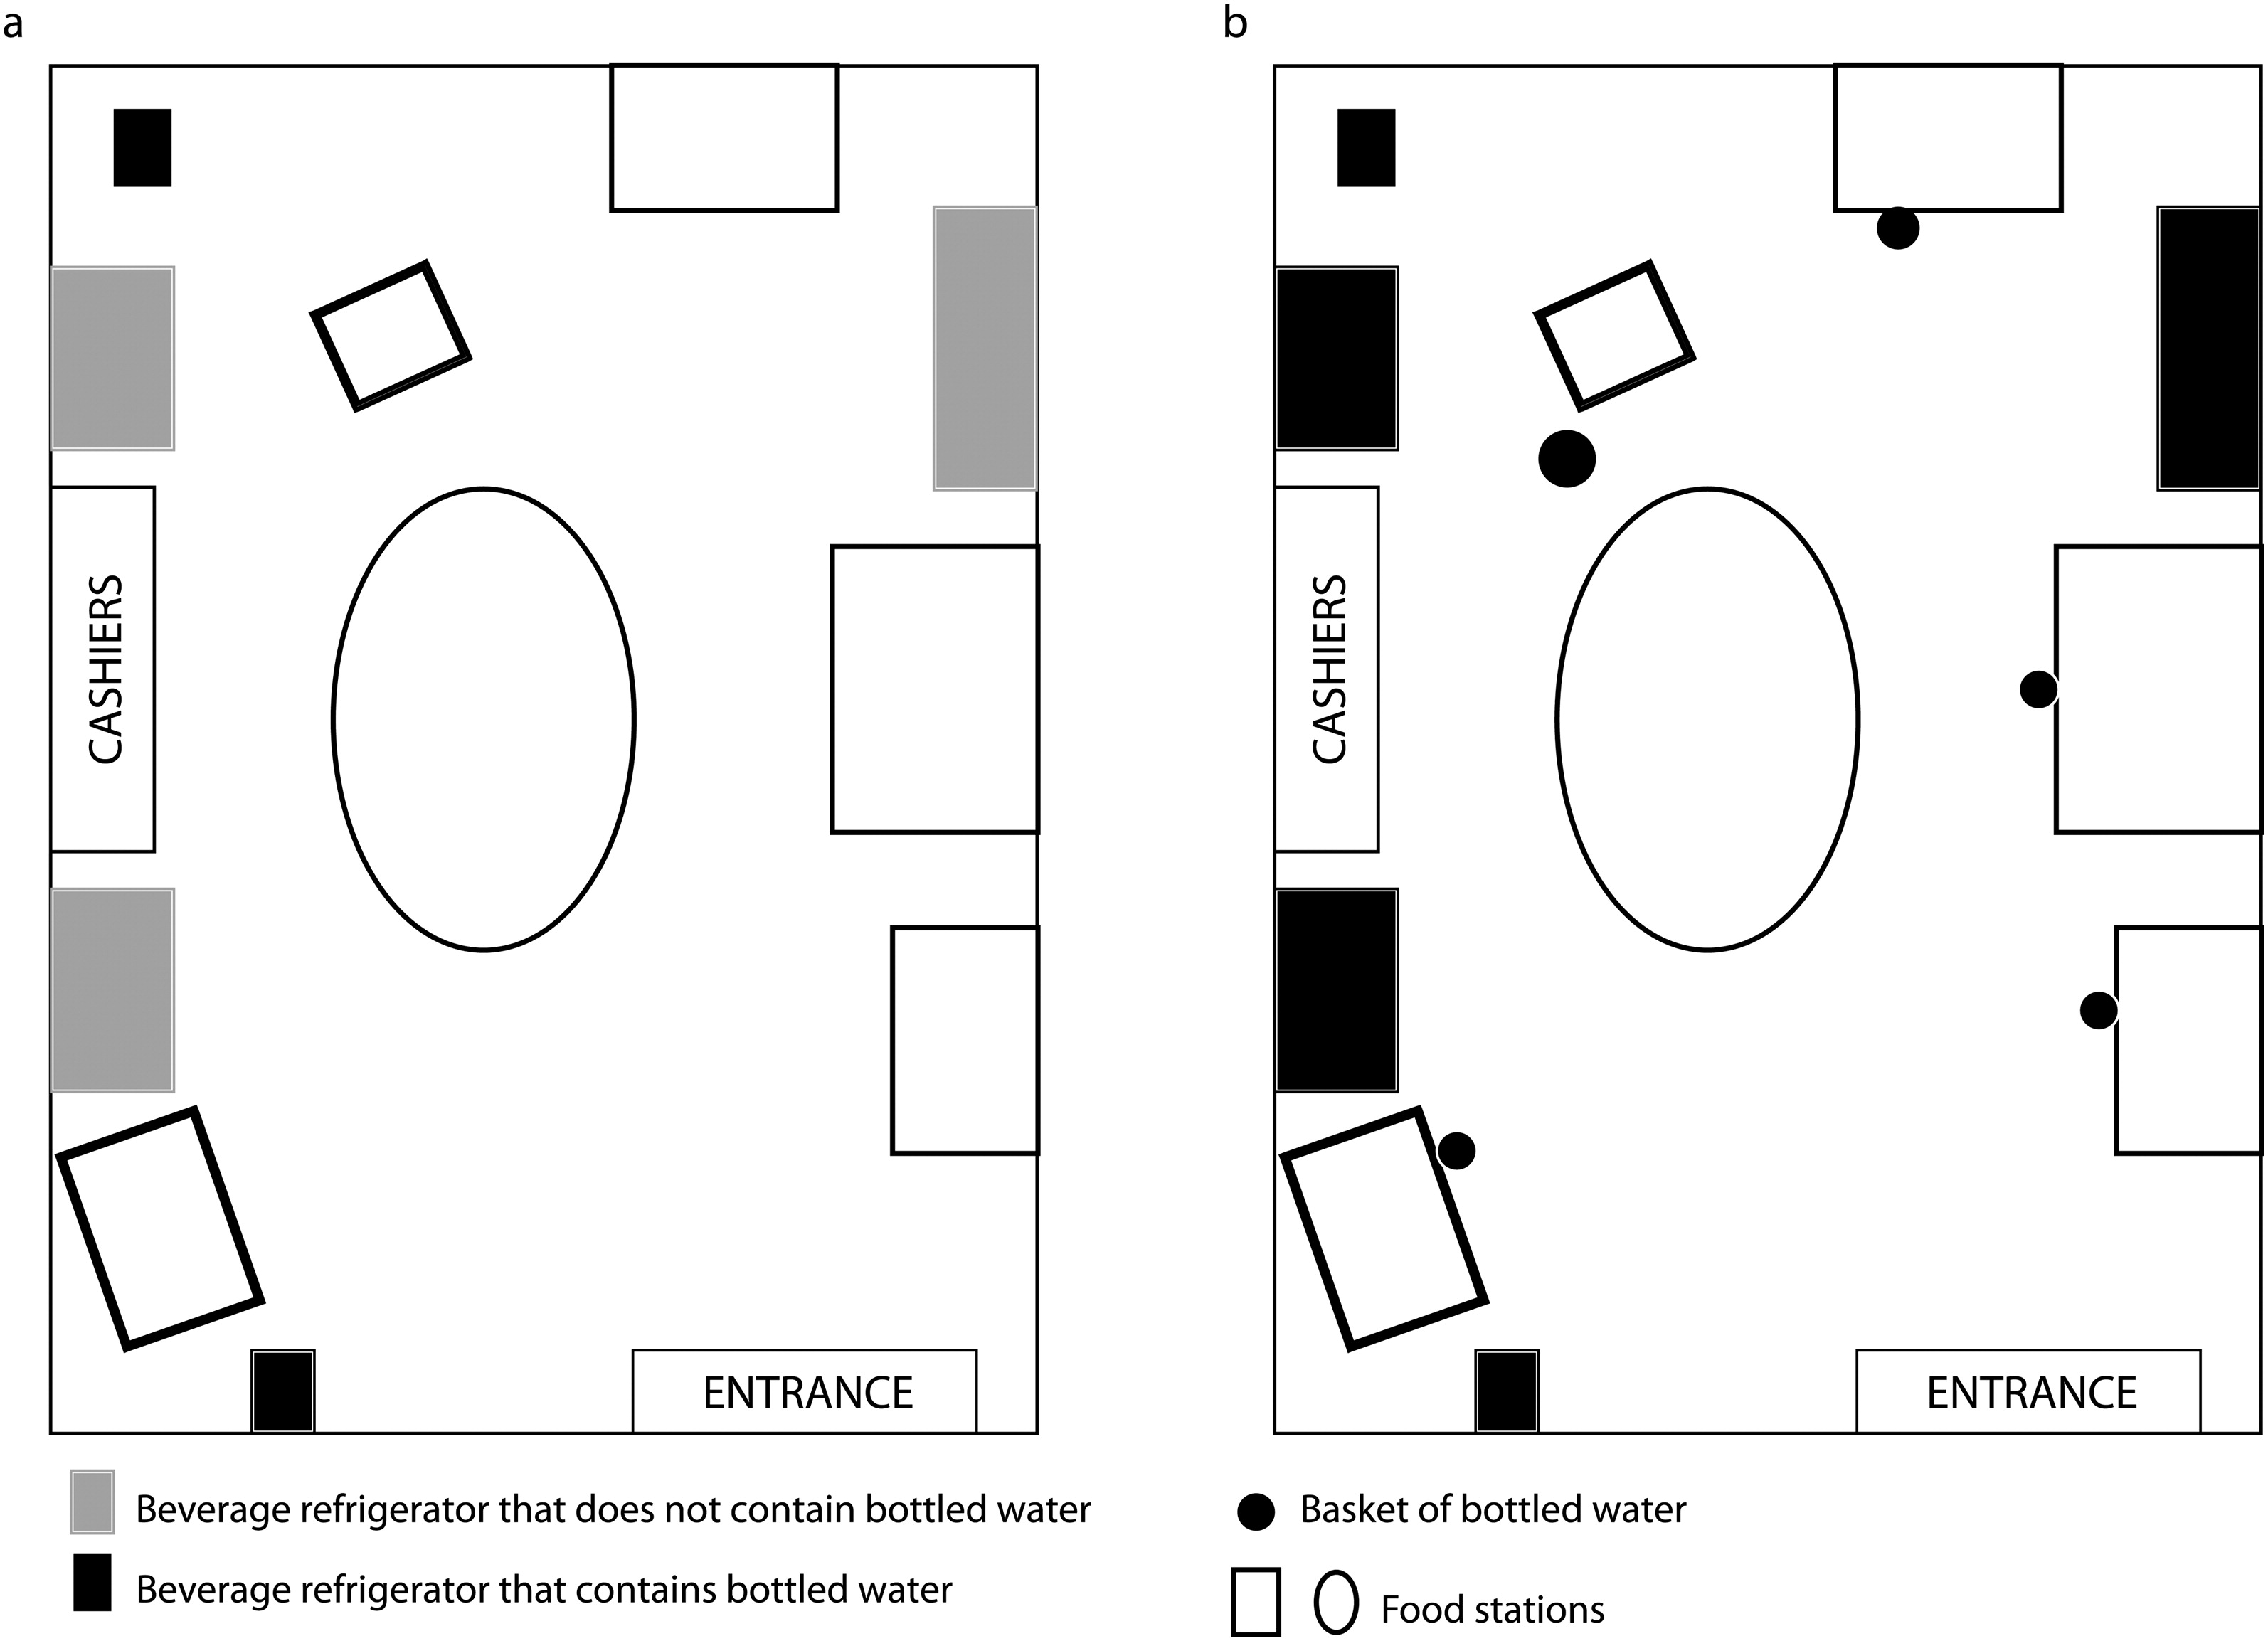
\includegraphics[width=\linewidth]{figures/thorndaik_architecture_choice.jpeg}
  \caption{Картинка «a» показывает, как выглядело помещение до изменений, а картинка «b» — после изменений. Источник: American Journal of Public Health, April 2012}
  \label{fig:pic1}
\end{figure}

Эффективность формирования привычек также можно повысить с помощью «архитектуры выбора» («choice architecture»). Этот подход основан на управлении окружением и организации условий таким образом, чтобы предпочтительное поведение стало максимально лёгким и естественным, а нежелательное – наоборот, сложным и неудобным \cite{thaler_nudge_2008}. Торндайк и её команда провели исследование, чтобы изменить расположение продуктов в кафетерии больницы. Они начали с того, что добавили воду в холодильники, которые раньше были заполнены только газировкой, и поставили корзины с бутылками воды рядом с едой в разных частях кафе. Таким образом, вода стала доступна везде, где были напитки, в то время как газировка осталась в тех же холодильниках (рис. \ref{fig:pic1}). Похожие изменения были внесены и в расположение еды. В результате продажа вредных напитков уменьшилась на 11,4\%, а продажа бутылок с водой увеличилась на 25,8\% \cite{thorndike_2012}.

Если реализационные намерения и архитектура выбора помогают связать поведение с контекстом, то позитивное подкрепление увеличивает вероятность, что поведение будет повторяться. Позитивное подкрепление (positive reinforcement) — это подход, основанный на принципах оперантного обусловливания, где поведение закрепляется за счёт последующего позитивного подкрепления – награды, одобрения или других приятных последствий \cite{Skinner1953}. Например, предоставление человеку награды после выполнения действия (даже символической, такой как похвала или отметка в дневнике достижений) существенно увеличивает вероятность повторения этого поведения в будущем. Удовольствие и внутренняя мотивация не только побуждают людей повторять нужное поведение, но и делают каждое повторение более эффективным для формирования привычки \cite{Landry2019Positive}. Этот эффект наблюдается в различных видах активности — от использования зубной нити и приёма витаминов до физических упражнений \cite{Judah2018Exploratory, Fremling2025Comparing, Wiedemann2014Intrinsic}.

Вышеперечисленные подходы в той или иной мере действенны и используются на практике. Есть и другие подходы, которые автор не стал упоминать из-за того, что они не так часто применяются в формировании привычек. Например, в таксономии техник изменения поведения насчитывается 93 техники, объединенных в кластеры \cite{michie_2008_bct}. Также имеется более современная версия таксономии с 281 техникой \cite{ontology_bct}. Каждая из этих техник теоретически может быть применена для формирования привычек, поскольку привычка — это вид поведения. Тем не менее, в научных исследованиях, посвященных формированию привычек, эти техники упоминаются достаточно редко.

Автор также не стал углубляться в теории изменения поведения и формирования привычек, такие как теория самодетерминации, модель COM-B, поведенческая модель Фогга, Habit Loop, теория запланированного поведения, транстеоретическая модель и прочие. Для понимания процесса формирования привычек подобные теории несомненно важны. Но для непосредственно создания привычек вряд ли эти теории более полезны, чем практические подходы и методы. Тем не менее, некоторые из этих теорий будут кратко упомянуты ниже — исключительно в качестве пояснительного контекста к описываемым методам. Более подробный разбор основных теорий и их применения для формирования привычек с использованием цифровых инструментов представлен в работе К. Пиндера и соавторов \cite{10.1145/3196830}.

Особенность рассмотренных подходов состоит в том, что они известны, как правило, в научной и «околонаучной» среде. На взгляд автора, это связано с тем, что эти подходы кажутся довольно «точечными», и мало известно о том, как они связаны с другими подходами, не говоря уже о том, чтобы они были увязаны в некий единый и понятный для широкой публики алгоритм. Ситуация с теориями еще сложнее, поскольку часто неясно, как применять их на практике. Это замечание особенно справедливо для описательных теорий, таких как теория самодетерминации, и менее справедливо для процедурных теорий, таких как модель Фогга или COM-B.

Наиболее известны три попытки популяризации поведенческой науки о формировании привычек для широкого круга читателей.

Первое издание «The Power of Habit» было опубликовано в 2012 году. Автор Чарльз Дахигг — журналист, а не эксперт в области нейробиологии или психологии, однако его модель Habit Loop обрела широкую известность, в том числе и в научной среде. Согласно этой модели, привычка формируется через цикл из трёх компонентов: сигнала (cue), поведения (routine) и вознаграждения (reward) \cite{duhigg_power_2012}. Важным дополнением к этому циклу является компонент «craving» (желание), который Дахигг вводит между сигналом и поведением. Это ощущение ожидания удовольствия, которое возникает в ответ на сигнал и предшествует выполнению рутинного действия. Процесс работает следующим образом: сигнал запускает желание (craving), которое, в свою очередь, побуждает к выполнению действия (routine). Это поведение закрепляется за счёт вознаграждения, которое служит подтверждением правильности выбора. Многократное повторение цикла способствует укреплению нейронных связей и закреплению привычки. Основная мысль — создать цикл, в котором сигнал запускает рутину, которая затем подкрепляется наградой. Несмотря на подробное и понятное описание процесса формирования привычек, в книге немного практических рекомендаций по внедрению этой модели в повседневную жизнь.

Широкую популярность получила книга «Atomic Habits» Дж. Клира, опубликованная в 2018 году, которая в том же году стала международным бестселлером \cite{noauthor_avery_nodate, editor_james_2022, bureau_james_nodate}. В отличие от «The Power of Habit», эта книга ориентирована на практическое применение принципов формирования привычек. В ней предлагаются четыре «закона» создания привычек: сделать поведение очевидным, привлекательным, легким и приятным \cite{clear_atomic_2018}. Можно сразу заметить, что эти четыре закона соответствуют циклу привычки Дахигга «cue-craving-routine-reward». Клир встраивает в этот цикл уже упомянутые выше научные подходы — реализационные намерения, архитектуру выбора, позитивное подкрепление, якорение, а также некоторые техники изменения поведения вроде self-monitoring of behavior (BCT 2.3). Для долгосрочного закрепления привычек Клир предлагает формирование привычек, основанных на идентичности. Согласно этому подходу, наиболее устойчивые привычки возникают тогда, когда поведение связано с самоощущением человека и его идентичностью. Например, человек, который считает себя спортсменом, с большей вероятностью будет регулярно заниматься спортом, поскольку это поведение является частью его личной идентичности. На официальном сайте Дж. Клира есть ссылка на мобильное приложение «Atoms», которое основано на системе «Atomic Habits» \cite{noauthor_atoms_nodate}.

Метод «Tiny Habits» был разработан Б.Дж. Фоггом, специалистом по поведенческим наукам, и впервые был представлен в 2019 году в его книге «Tiny Habits: The Small Changes That Change Everything» \cite{phd_tiny_2020}. Однако сам метод начал развиваться гораздо раньше — Фогг изучал поведенческие изменения и психологию людей более 20 лет, прежде чем официально представил свою методику \cite{noauthor_tiny_nodate}. Основная идея заключается в том, чтобы выбирать маленькие, простые действия и связывать их с уже существующими привычками \cite{noauthor_bj_nodate}. В «Tiny Habits» используются те же научные подходы, что и в «Atomic Habits», однако способ их применения существенно различается.

Начнем с того, что в «Atomic Habits» практически не затрагивается вопрос выбора привычек. Подразумевается, будто человек уже заранее знает, какую привычку хотелось бы ему привить. В «Tiny Habits» первоочередное внимание уделяется не просто выбору подходящей привычки, а прояснению «стремления» (aspiration) — той цели, ради которой человек готов меняться. Далее предлагается «мозговой штурм», в ходе которого необходимо придумать как можно больше вариантов поведения для достижения стремления. Эти варианты сортируются по трем критериям: желания и возможности выполнять поведение, а также эффективности поведения в достижении стремления. Выбирается та привычка, которая наиболее удовлетворяет перечисленным критериям. Такой подход усиливает внутреннюю мотивацию, поскольку выбор основан на личной значимости и высокой воспринимаемой полезности.

Следующее отличие состоит в том, что «Atomic Habits» основан на модели Habit Loop, в то время как «Tiny Habits» основан на собственной поведенческой модели. Поведенческая модель Фогга состоит из трех компонентов: мотивация (motivation), способность (ability) и подсказка (prompt). Согласно модели, поведение происходит только тогда, когда вместе соединяются все эти три компонента \cite{fogg_2009}. Фогг рекомендует уделить особое внимание способности — сделать поведение настолько легким, насколько это возможно \cite{phd_tiny_2020}. Сложность поведения зависит от пяти факторов: время, деньги, физические усилия, ментальные усилия и соответствие текущей рутине. Чтобы сделать поведение проще, нужно сначала выяснить, какой или какие из этих факторов делают поведение сложным, а затем можно снижать значимость этих факторов тремя способами: развивая навыки, используя вспомогательные инструменты, либо максимально упрощая само действие. Последнего можно добиться, разбив действие на микрошаги (например, вместо пробежки просто надеть кроссовки) или уменьшив его объем (например, сделать 2 отжимания вместо 20). После того, как поведение упрощено, требуется выбрать подсказку с помощью якорения. К слову, метод якорения в контексте формирования привычек был разработан именно Фоггом на основе предыдущих исследований, о чем упоминает Дж. Клир в своем блоге и в примечаниях к «Atomic Habits» \cite{clear_how_2014, clear_atomic_2018}.

Другое отличие заключается в том, что «Tiny Habits» предлагает «репетиции». После определения целевого поведения и подсказки предлагается сознательно повторить действие 7-10 раз подряд. Например, для «рецепта» привычки «после того, как я встаю с кровати, я делаю два отжимания», алгоритм будет следующим: (1) сесть на кровать, (2) встать, (3) выполнить два отжимания, (4) мысленно похвалить себя — и повторить всю последовательность 7-10 раз. Репетиции укрепляют нейронные связи, тем самым поведение становится более автоматичным. Так повышается устойчивость привычки и облегчается её выполнение в дальнейшем.

\begin{figure}[h]
  \centering
  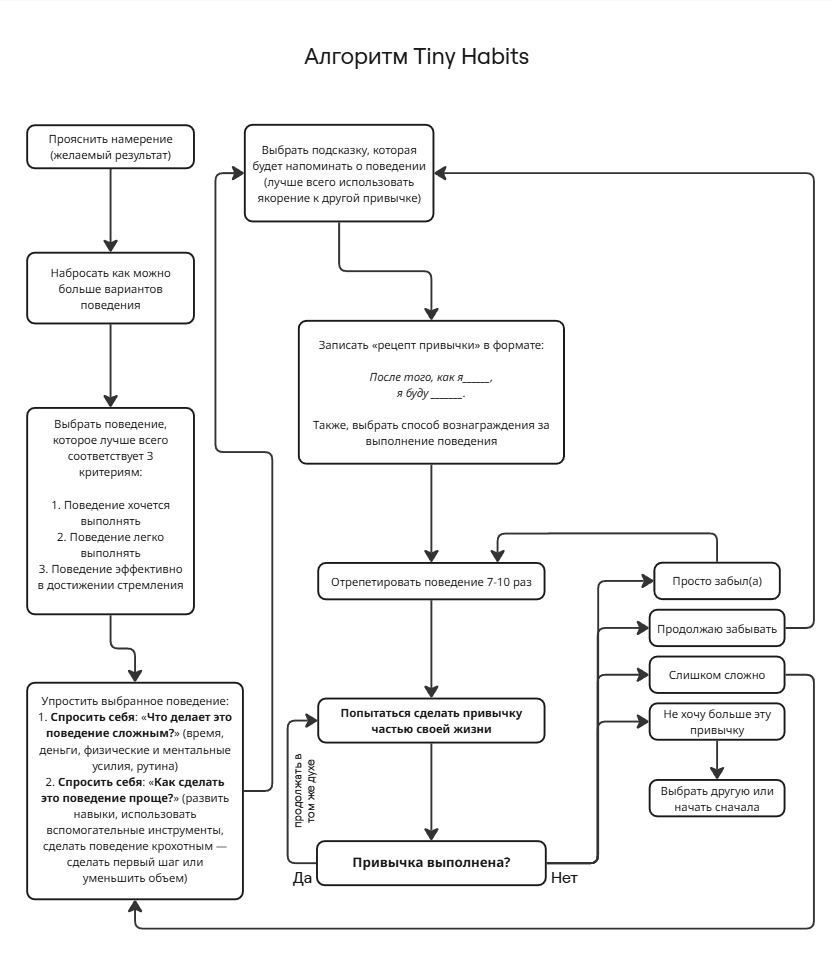
\includegraphics[width=\linewidth]{figures/tiny_habits_alg.jpg}
  \caption{Алгоритм «Tiny Habits». Составлено автором по книге «Tiny Habits» (2020)}
  \label{fig:pic2}
\end{figure}

Метод «Tiny Habits» выделяется среди других методов и научных подходов своей ярко выраженной практической направленностью.  По мнению автора данной работы, советы и инструкции, представленные в «Tiny Habits», более последовательны и ясны, чем у других подходов. Именно этот метод предлагает конкретный и понятный алгоритм формирования привычек (рис. \ref{fig:pic2}). Прочие подходы либо узконаправленные и затрагивают какой-то один аспект формирования привычек (например, реализационные намерения помогают соединить поведение с контекстом, а позитивное подкрепление выступает в роли катализатора), либо носят описательный характер (теории вроде Habit Loop), либо представляют собой перечень советов по формированию привычек (Atomic Habits).

Несколько исследований указывают на потенциальную эффективность метода «Tiny Habits» в формировании устойчивых привычек. Так, РКИ, посвященное влиянию «Tiny Habits» на благодарность, показало, что у участников, которые сосредоточились на культивировании благодарности с помощью маленьких привычек, значительно улучшились показатели самооценки благодарности, причем эффект сохранялся до одного месяца \cite{Hollingsworth2022Tiny}. Аналогично, пилотный эксперимент в области устойчивого потребления показал, что «Tiny Habits» способствует долгосрочному сохранению экологичных привычек \cite{OHalloran2024Small}. Еще одно исследование продемонстрировало эффективность поведенческих вмешательств, основанных на «Tiny Habits», для улучшения контроля за гликемией у пациентов с диабетом в Саудовской Аравии \cite{alqutub_2025}. Автору данной работы неизвестно о существовании других исследований, оценивающих эффективность метода «Tiny Habits», однако предыдущие работы показывают, что легковыполнимые действия с большей вероятностью становятся привычными \cite{lally_2010, https://doi.org/10.1348/014466605X49122}, так же, как действия, основанные на внутренней мотивации \cite{Judah2018Exploratory, phillips_2016}.

Хотя «Tiny Habits» показывает высокий потенциал в некоторых областях, его универсальность и долгосрочное влияние на различные типы поведения не доказаны. Кроме того, автор метода утверждает, что «Tiny Habits» был основан не столько на академической литературе, сколько на исследованиях самого автора \cite{tiny_habits_references}. Эти исследования являются частью курса Фогга «Tiny Habits», который был запущен в 2011 году, но при этом их результаты не были опубликованы. В настоящее время курс «Tiny Habits» проводится на коммерческой основе и название «Tiny Habits» является зарегистрированным товарным знаком \cite{noauthor_bj_nodate, noauthor_permissions_nodate}. Непрозрачность метода при довольно сильной коммерциализации лишний раз подчеркивает необходимость всесторонней оценки его эффективности.

\subsection{Обоснование значимости работы и ее цель}\label{Goal}

Пробел в научных знаниях и значимость данной работы можно сформулировать так.

Формировать полезные привычки важно, но в процессе люди часто сталкиваются с препятствиями. Для их преодоления существует множество подходов, из которых наиболее известны реализационные намерения, якорение, позитивное подкрепление и архитектура выбора. Эти подходы помогают связать целевое действие со стимулом (контекстом) и увеличить вероятность многоразового повторения этого действия в ответ на стимул, что, в итоге, должно привести к автоматической реакции — формированию привычки. Существуют также и методы, которые увязывают эти и другие подходы в некую систему. Наиболее известны две таких системы — «Atomic Habits» и «Tiny Habits», причем последняя примечательна своей исключительной практической направленностью и последовательностью. Несмотря на популярность метода и его высокий потенциал, эффективность «Tiny Habits» в формировании привычек почти не исследована. В качестве инструмента для вмешательств лучше всего подходят смартфоны из-за их распространенности, доступности и возможностей персонализации. Существует множество мобильных приложений по формированию привычек, однако их эффективность остается невыясненной и большинство из них не используют научные подходы и методы.

Таким образом, \textbf{цель работы} — разработать прототип мобильного приложения для формирования привычек на основе метода «Tiny Habits».

На основе прототипа разработчики смогут создать приложение, которое поможет:

\begin{enumerate}
    \item Отслеживать и формировать привычки (для конечных пользователей)
    \item Оценить эффективность метода «Tiny Habits» (например, с помощью экспериментов или анализа исторических данных)
    \item Оценить эффективность приложения как инструмента, содействующего в формировании привычек
\end{enumerate}

\textbf{Целевая аудитория приложения (ЦА)} — взрослые русскоговорящие пользователи, заинтересованные в саморазвитии и формировании привычек. К ЦА не относятся пользователи с серьезными зависимостями (например, табачной или наркотической), а также пользователи, которые желают значительных перемен в своем образе жизни. Причина исключения состоит в том, что первым требуется профессиональная помощь, а вторым необходимы более интенсивные вмешательства.

\subsection{Структура}\label{Structure}

Основная часть работы состоит из трех разделов: 1) контекст и потребности, 2) разработка решения, 3) итоговое оценивание. В начале каждого раздела ставятся исследовательские вопросы, выбираются подходящие методы для ответа на них, а в конце формулируются выводы и обозначаются ограничения. В заключительной части обсуждаются общие выводы, а также предлагаются практические рекомендации и дальнейшие направления исследований.

\newpage

\section{Контекст и потребности}\label{Context and Needs}

\subsection{Обзор раздела}\label{Overview1}

Люди пользуются продуктами и сервисами, когда эти продукты и сервисы удовлетворяют их потребности. Стало быть, прежде чем разрабатывать приложение, нужно выяснить, чего хотят люди и при каких обстоятельствах.

\bigskip
Исследовательские вопросы раздела:

\begin{itemize}
    \item В чем состоят характеристики целевой аудитории?
    \item Какие у нее потребности? При каких обстоятельствах эти потребности проявляются?
    \item Какие из этих потребностей наиболее важные?
    \item Что уже сделано для решения потребностей?
\end{itemize}

Исходя из исследовательских вопросов, были выбраны исследовательские методы и соответствующие UX-артефакты (см. таблицу \ref{tab:table1}).

\begin{table}[h]
\normalsize
\caption{Методы исследования, ключевые вопросы и артефакты}
\label{tab:table1}
\begin{tabular}{|l|p{5cm}|p{5cm}|}
\hline
\textbf{Метод}           & \textbf{Вопрос(ы), соответствущий(-е) методу}                                                                                  & \textbf{Артефакты}                                      \\ \hline
\textbf{Интервью}        & В чем состоят характеристики ЦА? \newline Какие у нее потребности? \newline При каких обстоятельствах эти потребности проявляются? & User Stories \newline Job stories                \\ \hline
\textbf{Опрос}           & Какие потребности самые важные?                                                                                                & Отчет по результатам опроса \newline Визуализация данных \\ \hline
\textbf{Конкурентный анализ} & Что уже сделано для решения потребностей?                                                                                      & Отчет об эвристической оценке                            \\ \hline
\end{tabular}
\end{table}

Ответив на обозначенные исследовательские вопросы, мы сможем сформулировать требования к мобильному приложению.

\subsection{Интервью}\label{Interview}

Итак, первая задача состоит в том, чтобы определить характеристики ЦА и ее потребности, которые потенциально могут влиять на использование приложения. Для этой задачи подходит интервью, поскольку этот метод широко применяется на ранних стадиях процесса UCD (User-Centered Design) и помогает исследователям понять, что нужно пользователям и с какими трудностями они сталкиваются в повседневной жизни \cite{LAZAR2017187, user_interviews}. 

\subsubsection{Участники}

Ранее мы определили целевую аудиторию как взрослых русскоговорящих людей, заинтересованных в саморазвитии и формировании привычек, за исключением людей с серьезными зависимостями и тех, кто желает значительных перемен. Естественное место, где можно найти таких людей — группы по саморазвитию, в которых периодически выкладываются материалы по внедрению полезных привычек.

Всего было рекрутировано 10 участников. Процесс рекрутинга состоял в следующем. Проявившим определенную активность (например, реакции или комментарии в ответ на пост) в тематических группах ВК и Телеграм-каналах рассылались приглашения на интервью через систему личных сообщений (ЛС). Один Телеграм-канал был посвящен мобильному приложению по формированию привычек «Habitica». Из этого канала было рекрутировано 2 участника — мужчина и женщина. Специальных критериев включения и исключения участников не было. Каждому участнику предлагалось вознаграждение — 40 электронных книг и 18 аудиокниг по саморазвитию.

\subsubsection{Процедура}

Исследование было направлено на то, чтобы изучить опыт людей в формировании привычек, а также то, как этот опыт соотносится с использованием технологий и инструментов для решения такой задачи. Под «технологиями» и «инструментами» подразумеваются не только мобильные приложения, но и десктопные приложения, веб-сайты, блокноты, будильники, календари; словом, все те продукты человеческой мысли, которые помогают внедрять привычки.

Интервью проводилось онлайн, в полуструктурированном формате и занимало около 40—60 минут. Все участники дали устное разрешение на запись. Им были заданы вопросы, касающиеся их самих (например: чем занимаются, какие привычки хотели бы сформировать), опыта и контекста формирования привычек (как пробовали внедрять привычки в прошлом, что работало, что не работало, какие привычки давались легче или труднее и т.п.), а также инструментов для формирования привычек (например: чем пользовались, как часто, что помогало и каким образом). Двум пользователям «Habitica» задавались дополнительные вопросы про приложение, а также им предлагалось продемонстрировать экран и показать, как они используют это приложение на практике. В таблице \ref{tab:table2} показана структура интервью и некоторые из заданных вопросов (поскольку интервью было полуструктурированным, у автора данной работы сохранялось право отходить от плана и задавать уточняющие вопросы).

\begin{table}[]
\normalsize
\caption{Структура интервью}
\label{tab:table2}
\begin{tabular}{|l|l|l|}
\hline
\textbf{Тема} &
  \textbf{Вопросы и предметы обсуждения} &
  \textbf{Длительность} \\ \hline
Вступление &
  \begin{tabular}[c]{@{}l@{}}Благодарность за участие\\ О чем это интервью и что от него ожидать\\ Согласие на запись\\ —Есть ли у вас вопросы, прежде чем мы начнем?\end{tabular} &
  5 мин \\ \hline
Биография &
  \begin{tabular}[c]{@{}l@{}}—Пожалуйста, расскажите немного о себе.\\ —Чем вы занимаетесь или чем любите заниматься?\end{tabular} &
  5 мин \\ \hline
Привычки &
  \begin{tabular}[c]{@{}l@{}}—Какие привычки вам хотелось бы сформировать\\ (или от каких избавиться)? Почему?\\ —Приходилось ли вам внедрять полезные привычки?\\ Что это были за привычки и как вы их внедряли?\\ —С какими сложностями сталкивались?\\ —Как вы напоминаете себе о привычках?\\ —При каких обстоятельствах вы пропускаете\\ выполнение привычки? Что вы чувствуете?\\ —Как ваш круг общения (семья, друзья, знакомые)\\ влияют на ваши привычки?\\ —Было ли такое, когда поддержка со стороны\\ близких не помогла или даже навредила\\ вашим усилиям?\\ —Как вы относитесь к тому, чтобы делиться своими\\ целями и успехами с другими людьми?\end{tabular} &
  10-15 мин \\ \hline
Инструменты &
  \begin{tabular}[c]{@{}l@{}}—Использовали ли вы какие-нибудь инструменты\\ для отслеживания привычек? Если да, то какие?\\ —Расскажите про ваш опыт использования \\ такого-то инструмента\\ —Что, в целом, думаете про ваш опыт?\\ \\ Доп. вопросы про приложение:\\ —Почему решили выбрать это приложение?\\ —Как вы записываете привычки в приложении?\\ —Не могли бы вы пошагово показать, как вы \\ используете это приложение?\\ —Какими функциями вы чаще всего пользуетесь?\\ —С какими трудностями сталкиваетесь?\\ —Что вам нравится в этом приложении? Почему\\ до сих пор используете его?\end{tabular} &
  10-15 мин \\ \hline
Завершение &
  \begin{tabular}[c]{@{}l@{}}—Прежде чем мы закончим, не хотите ли еще чего-то\\ добавить?\\ —Не могли бы вы сказать свой возраст или \\ возрастную группу?\\ Благодарность, завершение интервью\end{tabular} &
  5 мин \\ \hline
\end{tabular}
\end{table}

\subsubsection{Анализ данных}

Для анализа и интерпретации данных был проведен тематический анализ. Это стандартная практика, применяемая для анализа качественных данных \cite{Majumdar2019Thematic}. Использовался 6-шаговый процесс, предложенный В. Браун и В. Кларк: 1) ознакомление с данными, 2) генерация первоначальных кодов, 3) поиск тем, 4) обзор тем, 5) определение и наименование тем, 6) написание отчета \cite{Clarke2017Thematic}.

\subsubsection{Результаты}

Благодаря тематическому анализу, были выявлены три мегатемы — персона, привычки и инструменты. Особняком стояла тема «коучинга» — использования приложения для обучения формированию полезных привычек клиентов.

\textit{Персона: демография}. В интервью участвовали люди от 19 до 48 лет. Среди них было трое мужчин (22, 38 и 40 лет) и семь женщин (19, 31, 33, 40, 40, 47 и 48 лет). Почти все респонденты старше 30 лет, за исключением двоих, состояли в семье и имели детей. Род деятельности участников оказался разнообразным: тренер по горным лыжам, анестезиолог-реаниматолог, студентка-психолог, исполнительный директор на предприятии, фермер, владелец малого бизнеса и председатель Общественной палаты, профессиональный коуч в области отношений и восстановления пищевого поведения, фрилансер в дизайне, коммьюнити-менеджер в игровой компании, разработчик ПО в международной компании.

\textit{Персона: интересы и увлечения}. В целом, большинству участников нравилось ходить в тренажерный зал, путешествовать, смотреть каналы на YouTube по теме саморазвития, психологии, личностного роста. Один участник увлекался нейрофизиологией, рисованием и учил немецкий. Другая участница увлекалась психологией и обучалась в онлайн-университете ради дополнительной специализации. 

\textit{Персона: мотивация}. Многие участники решили начать меняться, потому что чувствовали, что их что-то не устраивает в себе. «\textit{Вот я не тренировался порядка трех лет. Из-за этого я потерял форму, набрал массу. То есть все физические параметры были снижены прям до нуля, как в компьютерной игре, и их нужно было как-то прокачивать}». «\textit{Перестала нравиться себе в том плане, что как кошка домашняя стала. Чувствовала себя немножко расплывчатой...}». Некоторых участников вдохновлял пример других людей. Одна из участниц таким образом решила начать регулярно пить воду: «\textit{Я просто видела опыт других людей, что они пьют, и хотела попробовать также. Вроде как это интересная привычка, но она как-то не совсем прижилась}». Другая участница знала о полезности привычки пить воду, это было в ее целях, но начала она только «за компанию». Еще одна участница считала важным получить аргументированное обоснование привычки, прежде чем ее внедрять: «\textit{Если просто скажут: "это классно, это полезно" — это не работает. А если есть именно какая-то информация, которая заставляет задуматься, что это полезно для здоровья, [...], то это самое эффективное и действенное}». Некоторые отмечали колебания мотивации: «\textit{Часто было такое, что сначала как бы ты замотивируешься что-то изменить или какие-то привычки новые привить. И эта мотивация длится не очень долго. То есть неделю может длится, но потом, как правило, это все спадает. И вот там как раз наступает момент, когда ты либо можешь взять себя в руки и идти дальше, либо ты сдаешься и опять заново потом начинать. У меня такое часто было со спортом, что я начинала, могла даже месяц заниматься регулярно, потом опять забрасывала}». Одна участница связала это с тем, что не было конкретной цели и понимания, зачем нужна эта привычка. Участники по-разному относились к краткосрочным и долгосрочным результатам. Для одних важен сам процесс: как выразился один участник, «\textit{у самурая нет цели, есть только путь}» — результаты становятся заметны лишь со временем, «\textit{здесь подвырос, там подвырос, и просто двигаешься дальше}». Для других же важна быстрая отдача: например, одна участница призналась, что, если не замечает эффектов от новой привычки в течение трёх-четырёх недель, начинает сомневаться в её эффективности и может отказаться от её дальнейшего выполнения.

\textit{Персона и сообщество}. Участники хотели делиться своими успехами, чтобы вдохновлять других людей и передавать свой опыт, чтобы другие люди совершали меньше ошибок. Кому-то из участников в принципе не хотелось ничем делиться. Кто-то хотел делиться своими успехами с близкими подругами или когда спросят. В целом, роль сообщества в формировании привычек считалась важной. Так, участница-предприниматель приводила в пример поговорку: «\textit{хочешь летать с орлами, не пасись с индюками}». Участник-фермер привел пример знакомого, который «слез с героина» из-за того, что тот присоединился к сообществу анонимных наркоманов. Сам фермер утверждал, что перестал курить, когда ушел из курящего окружения. Участница-студентка устраивала соревнования с подругой: «\textit{Каждый день докладывали друг другу, что делали, сколько позанимались, снимали видео. Потому что если ты проиграешь, то надо будет сделать что-то не очень приятное. Это мотивировало заниматься спортом месяц}». Другая участница записывала «Дневник успеха». Это чат в Telegram, в котором она и ее подруга делились своими успехами за день. Участница отмечала, что это поднимает мотивацию, однако если подруга не сделала ничего, то мотивация снижалась – «\textit{ну я в принципе тоже могу ничего не делать}». Для этой же участницы было важно найти людей примерно одного уровня с общими целями и интересами. Сообщество со значительно более высоким уровнем демотивировало: «\textit{я такой нуб среди них и не очень вписываюсь}». Были примеры и негативного влияния сообщества — двое участников младше 30 не могли отказаться от сладкого, потому что родители покупали себе что-нибудь к чаю, и это лежало на видном месте. Участница постарше не смогла завязать с алкоголем, потому что ее приглашали подруги на вечеринки, но в то же время она не чувствовала неприятных последствий: «\textit{Когда наступают очередные выходные, когда звонят подруги, либо приглашают в кафе, либо это какие-то мероприятия, либо ещё что-то, я взвешиваю свое состояние. Оно мне никак не вредит. Оно не влияет на качество моей жизни. И вот опять куча отговорок. И все благополучно продолжается}.

\textit{Привычки: успешные примеры}. Одна участница рассказывала, что формирует привычки таким образом: сначала спрашивает себя «зачем она нужна?», потом ещё больше углубляется в «зачем» и пытается понять, что эта привычка ей даст, что она получит хорошего от этой привычки. После этого участница старается внедрить свою привычку и оценивает степень получаемого удовольствия от выполнения. Участница считала, что привычка должна быть «по кайфу» — которая «\textit{и закрывает цель, и тебе комфортна}». Другая участница сформировала свою полезную привычку случайно. Готовясь к ЕГЭ, она проводила много времени за компьютером и начала ставить рядом бутылку или стакан воды, попивая из него каждые 4–5 минут — просто от скуки. Со временем это действие стало привычкой. Ещё одна участница формировала привычки — или выполняла рабочие задачи — с помощью метода «героя»: она просто считала до трёх, а потом заставляла себя встать и начать действовать. Однако этот способ срабатывал не всегда (участница не смогла привести примеры). В целом участники отмечали, что привычки формируются легче, если они требуют минимальных затрат времени и усилий, заранее желанны и их приятно выполнять. Участники отмечали, что новое поведение легче закрепляется, когда оно вводится постепенно и в комфортных условиях — например, одна из участниц сдвигала время ужина поэтапно: с девяти на восемь, затем на семь, и в итоге на четыре часа дня, каждый этап был для неё посильным. Другой участнице удалось сформировать за счёт постепенного увеличения времени — по 2–3 секунды за раз. Такой подход позволял видеть небольшой, но ощутимый прогресс, что поддерживало мотивацию. Кроме того, устойчивость привычки усиливалась, если её выполнение вызывало положительные эмоции или, наоборот, сопровождалось дискомфортом при пропуске (хотя последнее, возможно, уже является следствием сформировавшегося поведения). Также важным условием было предварительное выделение времени на выполнение привычки, что помогало включить её в повседневный распорядок.

\textit{Привычки: барьеры на пути формирования}. Одна из участниц отмечала, что испытывает страх перед началом новой привычки из-за её высокой воспринимаемой сложности — особенно в тех случаях, когда хочется немедленного результата. У других участников наблюдался период адаптации или «ломки», который длился около недели-полутора. При этом для некоторых привычка становилась по-настоящему устойчивой только спустя значительное количество повторений — например, один участник отметил, что походы в спортзал начали восприниматься как неотъемлемая часть жизни только после примерно 80 тренировок. 

Новое поведение, по словам участников, не выполнялось по ряду причин. Во-первых, это могли быть внешние обстоятельства: занятость, отсутствие физической возможности, болезнь, отпуск, непредсказуемый график из-за маленьких детей или, например, посиделки с друзьями — так один из участников нарушил режим интервального голодания. Во-вторых, сказывалось внутреннее состояние: усталость, плохое самочувствие, ощущение разбитости. Также поведение откладывалось, даже если наступал «подходящий момент», но не было сформировано устойчивое внутреннее убеждение в необходимости действия — как в случае с участницей, которая всё время откладывала чтение стихов. 

Ещё одной частой причиной были когнитивные уловки: мысль вроде «ну ладно, один день пропущу» или «посмотрю одно видео — ничего страшного» сопровождалась внутренней борьбой между «ангелом» и «демоном», что в ряде случаев приводило к срыву.

Интересно, что краткосрочные пропуски не вызывали у участников сильного разочарования — они воспринимались как часть процесса, и важнее было «не провалиться в целом». Однако длительные перерывы, особенно вызванные накоплением сложностей, воспринимались болезненнее. Один из участников, например, рассказал, что из-за тяжёлой недели пропустил ведение дневника, и это стало началом цепочки пропусков — в итоге привычка была заброшена на два месяца. Другой участник упомянул, что после болезни и отпуска было сложно вернуться в привычный ритм, и восстановление поведения требовало дополнительных усилий.

\textit{Инструменты: выбор и виды} Участники применяли разнообразные инструменты — как цифровые, так и аналоговые — для поддержки формирования новых привычек. Среди них:

\begin{itemize}
    \item \textbf{Аналоговые средства}: бумажные блокноты, распечатанные календари и трекеры, где можно было отмечать выполнение действий.
    \item \textbf{Напоминания}: будильники с пояснительными подписями, уведомления на телефоне, заметки, всплывающие в нужное время.
    \item \textbf{Цифровые списки дел}: стандартные «To-do-листы» в телефоне или встроенные приложения для задач.
    \item \textbf{Приложения для формирования привычек}: специализированные сервисы, такие как FatSecret (отслеживание питания), приложение Митрошиной (по формированию привычек и трекингу задач), Habitica (геймификация привычек), Streaks, Tappsk и другие.
    \item \textbf{Органайзеры}: Obsidian, Notion, Evernote — использовались для систематизации задач, рефлексии и отслеживания прогресса.
\end{itemize}

Использование того или иного инструмента зависело от предпочтений участника, уровня его цифровой вовлечённости и целей, связанных с привычкой. Преимущества и недостатки инструментов, которые отмечали участники, приведены в таблице \ref{tab:table3}.

\begin{table}[]
\normalsize
\caption{Преимущества и недостатки избранных инструментов}
\label{tab:table3}
\begin{tabular}{|l|l|l|}
\hline
\textbf{Инструмент} &
  \textbf{Преимущества} &
  \textbf{Недостатки} \\ \hline
\begin{tabular}[c]{@{}l@{}}Бумажный \\ блокнот\end{tabular} &
  \begin{tabular}[c]{@{}l@{}}+Возможность «поставить плюсик» \\ и почувствовать момент «я это сделала»\\ +Маленький, легко носить с собой\\ +Можно отслеживать мысли нелинейно:\\ не только отслеживать привычку, но и\\ собственные размышления\\ +Тактильность\\ +Простота\end{tabular} &
  \begin{tabular}[c]{@{}l@{}}—Приходится отслеживать \\ прогресс вручную, \\ трудно строить графики\\ —Блокнот не сможет напомнить\\ о задаче, если о ней забыли\\ —Изнашивается при постоянном\\ использовании и переноске\\ —Требует регулярной замены\end{tabular} \\ \hline
\begin{tabular}[c]{@{}l@{}}Напоминания\\ (будильники)\end{tabular} &
  \begin{tabular}[c]{@{}l@{}}+Даёт возможность \\ распланировать день по блокам \\ и целенаправленно выделять время \\ на те сферы, которые хочется развивать\end{tabular} &
  \begin{tabular}[c]{@{}l@{}}—Могут приходить не вовремя и \\ тогда приходится их отключать\end{tabular} \\ \hline
\begin{tabular}[c]{@{}l@{}}Смартфон\\ (в целом)\end{tabular} &
  \begin{tabular}[c]{@{}l@{}}+Почти всегда под рукой\\ +Не зависит от качества бумаги, \\ типографии и других физ. ограничений\end{tabular} &
  \begin{tabular}[c]{@{}l@{}}—Риск «залипнуть»  и забыть, \\ зачем изначально его открывали\end{tabular} \\ \hline
\end{tabular}
\end{table}

Некоторые участники не использовали приложения для формирования привычек по разным причинам. Часть из них просто не знала о существовании таких цифровых инструментов, другим они казались слишком сложными и перегруженными. Были и те, кто в целом чувствовал себя неуверенно в цифровой среде: сами они не стремились осваивать новые приложения, но подчеркивали, что готовы выполнять инструкции, если им кто-то покажет, как этими приложениями пользоваться.

\textit{Инструменты: приложения для формирования привычек}. Участники отметили несколько ключевых особенностей, которые им особенно нравятся в мобильных приложениях. Среди них — настраиваемые уведомления, позволяющие получать точные и своевременные напоминания о делах. Отдельные участники положительно отзывались о функциях на базе машинного обучения, таких как прогнозирование событий на основе предыдущей активности (например, предсказание начала менструального цикла). Высоко ценится и быстрый поиск: достаточно ввести одну-две буквы, чтобы сразу увидеть нужный результат. Удобство интерфейса также играет важную роль — вся необходимая информация должна быть доступна на одной странице, без лишней навигации по меню и разделам. Простота, понятность и экономия времени были названы приоритетными требованиями. Кроме того, некоторым важно иметь возможность открыть календарь прямо в приложении, чтобы наглядно увидеть свои планы на день, неделю или месяц — это помогает оценить загруженность и спланировать время.

Среди неудобств, которые отмечали участники, выделяются как технические, так и пользовательские. Одним из часто упоминаемых недостатков было ограничение на количество задач в день — в некоторых приложениях, чтобы добавить более пяти дел, требовалась платная подписка. Участники подчеркивали сложность использования как один из главных недостатков многих приложений. Так, в одном из приложений необходимо было сначала пройти анкетирование, после чего приложение автоматически формировало список привычек. Однако из-за длительности этого процесса участница так и не дошла до этапа, где могла бы внести свои собственные привычки, потеряв мотивацию. Особенно часто упоминались навязчивые уведомления — они приходили в неподходящее время, например, когда пользователь был занят или телефон был разряжен. Вместо того чтобы стимулировать к действию, такие оповещения вызывали раздражение: хотелось не работать с привычками, а просто избавиться от этих уведомлений.

Пользователи удаляли приложения по целому ряду причин, связанных как с техническими ограничениями, так и с пользовательским опытом. Одной из распространённых причин было ощущение неполноценного доступа без оплаты: например, в приложении Forest для полноценного использования требовалась платная версия, при этом основная механика (выращивание дерева) легко обходилась, если просто свернуть приложение. Некоторые интерфейсы воспринимались как перегруженные и неудобные — с множеством таблиц, вкладок и переходов, требующих дополнительных усилий при использовании. Уведомления часто приходили в неподходящее время и воспринимались как навязчивые, вызывая раздражение. Отказ от приложений также происходил из-за излишней сложности — например, необходимости вручную вводить точные наименования продуктов или из-за чрезмерного количества рекламы. В ряде случаев приложения становились ненужными, поскольку нужные привычки уже были сформированы. Также отмечались такие технические проблемы, как баги (например, ошибки синхронизации между мобильной и десктопной версиями), торможение, чрезмерное потребление памяти устройства, а также ограниченный функционал, не соответствующий ожиданиям. Высокий порог входа, как в случае с Notion, делал начало работы трудным. Дополнительное беспокойство вызывали изменения ценовой политики и опасения, что компания может прекратить поддержку приложения или покинуть рынок.

Пользователи выделили ряд принципиально важных требований к приложениям, связанным с формированием привычек. Во-первых, ценится наличие бесплатной демо-версии — она позволяет понять функциональность и осознанно принять решение о покупке. Важно, чтобы интерфейс был максимально простым и понятным: всё нужное должно находиться "на виду", без лишних шагов и запутанных меню. Отдельное внимание уделяется приватности: трекеры не должны восприниматься как инструмент внешнего контроля — пользователь хочет быть уверенным, что его данные не просматриваются без согласия. Приложение должно предлагать простой, но эффективный путь к формированию привычек. Для пользователей старшего возраста особенно важны пошаговые инструкции, объясняющие, куда нажимать и что делать. Важно отслеживать прогресс — возможность оглянуться на месяц или год и увидеть, чего удалось достичь. Однако при слабых результатах статистика может вызывать разочарование, особенно если она не совпадает с изначальными ожиданиями пользователя. Также ценится визуальная узнаваемость — логотип приложения должен быть легко заметен на экране. Один из участников отметил, что дизайн мог бы отражать темы устойчивого развития, например, использовать зелёную цветовую палитру. Трекер привычек должен быть максимально прост: пользователь хочет быстро зафиксировать действие без долгих поисков. Дополнительной ценностью стало бы сообщество по интересам, где люди могли бы обсуждать свои привычки и поддерживать друг друга. При этом важно, чтобы пользователь чувствовал стабильность и контроль над своими данными — даже в случае технических сбоев или исчезновения приложения с рынка. Возможность создавать резервные копии рассматривается как необходимая мера безопасности.

\textit{Инструменты: Habitica}. Оба участника использовали Habitica преимущественно не как инструмент формирования привычек, а как средство для организации повседневных задач и тайм-менеджмента. Участница чаще всего работала с форматами to-do и dailies, используя приложение для записи конкретных дел, а не для отслеживания долгосрочных изменений поведения. Напоминания она устанавливала в основном для встреч. Участник продолжает пользоваться Habitica, несмотря на замеченные им недостатки, поскольку приложение стало частью его рутины: он привык к интерфейсу, знает, как с ним работать, и не хочет терять накопленных игровых питомцев, к которым сформировалась эмоциональная привязанность. Также он предпочитает десктопную версию Habitica — она позволяет удобнее печатать, копировать и вставлять тексты, а наличие постоянно открытой вкладки упрощает доступ к задачам в течение дня. 

Участники положительно оценили идею геймификации в Habitica. Им нравилось наблюдать, как развивается персонаж, открываются новые питомцы и становятся доступны рейды на боссов — это создавало дополнительную мотивацию и вовлечённость. Однако в процессе использования у них возникли и определённые трудности. Одним из главных неудобств стала невозможность задать гибкий график для привычек: если, например, привычку нужно выполнять трижды в неделю, то в остальные дни приложение всё равно требует какой-то активности — либо приходится вручную переносить задачу, либо отмечать её как невыполненную, что демотивирует. Также оба участника отметили нехватку функции бэклога — места, куда можно было бы сохранять задачи или мысли "на потом". Один из них пожаловался на то, что задачи и привычки нельзя внести списком, а приходится добавлять каждую вручную, что отнимает время. Кроме того, чаты сообщества перегружены системными уведомлениями — пользователям мешало большое количество сообщений о действиях других игроков (например, заклинаниях или уроне боссу). Отмечалась также нехватка поддержки для ведения более комплексных проектов с подзадачами, а также отсутствие календаря, в котором можно было бы отслеживать стрики. Участница призналась, что не до конца поняла, как использовать внутриигровые награды, а другой участник — что иногда прибегал к «читерству», отмечая старые невыполненные задачи, чтобы не подвести команду в квесте.

\textit{Дополнительная тема: коучинг}.  Одна из участниц, являющаяся профессиональным коучем в сфере отношений и восстановления пищевого поведения, не испытывала особенных затруднений с формированием собственных привычек. Вместо этого её интересовала другая задача — создание удобной системы взаимодействия с клиентами. Ей было важно, чтобы приложение помогало не только организовать личные задачи, но и поддерживать структуру работы с клиентами: фиксировать прогресс, отслеживать договорённости, вести заметки. Таким образом, запрос участницы выходил за рамки привычного использования приложений для личной продуктивности и предполагал их адаптацию под профессиональные нужды.

\subsubsection{Основные выводы}

Результаты интервью во многом согласуются с ключевыми положениями «Tiny Habits». Участники отмечали, что первоначальный порыв к изменениям (например, вызванный вдохновляющим видео) часто угасает уже через несколько дней. Это напрямую перекликается с подходом Б. Дж. Фогга: мотивация нестабильна и не может служить надежной опорой для устойчивых изменений поведения. Многие сталкивались с трудностями при формулировании целей и привычек: не всегда понятно, как именно описать желаемый результат. В такие моменты пользователи рассчитывают на поддержку со стороны приложения — вплоть до автоматических подсказок. Кроме того, часто возникала потребность в осмыслении пользы привычки: прежде чем начать её внедрение, человек хотел бы понять, действительно ли она приближает его к долгосрочным целям. Это также соответствует подходу Фогга, который предлагает сначала прояснить стремление, а уже затем подбирать подходящее поведение, исходя из его эффективности и выполнимости. Участники также подчёркивали, что легче всего внедряются привычки, которые максимально просты в исполнении и при этом приносят удовольствие. Это наблюдение полностью соответствует философии Tiny Habits: чем проще поведение, тем выше вероятность того, что оно произойдёт, а положительное подкрепление — ощущение пользы или удовольствия — помогает закрепить поведение и поддерживать интерес к нему.

Однако выявились и ограничения метода. Хотя «Tiny Habits» сосредоточен на создании устойчивых привычек за счёт их простоты, для некоторых участников очень важным оказалось быстрое получение ощутимого результата. Если в течение 2–3 недель не происходит заметных изменений, мотивация резко снижается. Это указывает на возможное расхождение между философией Tiny Habits, ориентированной на постепенные и малозаметные улучшения, и ожиданиями пользователей, стремящихся к быстрой поведенческой отдаче. Таким образом, метод может оказаться менее эффективным для тех, кто нуждается не только в формировании новой привычки, но и в явном подтверждении её ценности уже в краткосрочной перспективе.

На основе результатов интервью, можно сформулировать следующие Job Stories, которые могут лечь в основу проектирования приложения:

\begin{itemize}
    \item Когда я не знаю, как правильно сформулировать привычку или цель, я хочу, чтобы мне помогли (или сделали это за меня), чтобы не перегружать голову.
    \item Когда я хочу сформировать новую привычку, я хочу понять, действительно ли она мне нужна, чтобы идти к своей цели по верному пути и не тратить ресурсы впустую.
    \item Когда я выбираю привычку, я хочу найти такую, которая приносит максимальную пользу и при этом мне нравится, чтобы сохранялось желание продолжать.
    \item Когда я выбираю привычку, не требующую ежедневного выполнения, я хочу отмечать её только в нужные дни, чтобы видеть реальный прогресс и не сбивать статистику.
    \item Когда у меня нет телефона под рукой или он разрядился, я хочу помнить о своих привычках, чтобы выполнять их и не срываться.
    \item Когда я отмечаю выполнение своей привычки, я хочу иметь возможность записывать свои мысли в свободной форме, чтобы не забыть важные идеи или ощущения.
    \item Когда привычка кажется слишком сложной, я всё равно хочу её выполнять, чтобы быть ближе к своей цели.
    \item Когда я чувствую себя усталым или не в настроении, я хочу продолжать выполнять привычку, чтобы не срываться и сохранить устойчивость.
    \item Когда я сталкиваюсь с внутренней борьбой, я хочу выбрать полезное действие вместо вредного, чтобы быть ближе к своим целям и не мучиться угрызениями совести.
    \item Когда я вижу свой прогресс, я не хочу испытывать вину за промахи, чтобы сохранить внутреннюю опору и не снижать продуктивность.
    \item Когда я оцениваю свой прогресс, я не хочу, чтобы это возвращало меня к старому образу жизни, чтобы сохранить новые привычки и продолжать развиваться.
    \item Когда я на короткое время прерываю длинную серию выполнения привычки, я хочу продолжить её без сброса, чтобы не чувствовать поражение и сохранить мотивацию.
    \item Когда я поправился после болезни или выхожу из отпуска, я хочу вернуться к привычкам, чтобы восстановить продуктивный режим.
    \item Когда я хочу открыть приложение, я хочу видеть чёткое и узнаваемое лого, чтобы не путать его с другими и быстро его находить.
    \item Когда я беспокоюсь о сохранности данных, я хочу иметь возможность сделать резервную копию, чтобы не потерять информацию и прогресс.
    \item Когда я хочу ввести несколько привычек, я хочу вставить их списком, чтобы не тратить время на однотипные действия вручную.
\end{itemize}

Также, имеются потребности, которые связаны не столько с контекстом, сколько с самой персоной. Эти потребности сформулированы в виде User Stories:

\begin{itemize}
    \item Как родитель маленьких детей, я хочу иметь возможность выполнять привычку, несмотря на непредсказуемый график, чтобы продолжать быть продуктивным.
    \item Как неуверенный пользователь мобильных приложений, я хочу иметь понятную инструкцию, чтобы разобраться, как пользоваться приложением.
\end{itemize}

Некоторые потребности не были включены в списки выше по одной из двух причин: 1) нельзя удовлетворить с помощью мобильного приложения (пример: когда человек заходит в телефон, он хотел бы не отвлекаться на посторонние приложения); 2) были связаны с сообществом, что точно не будет входить в минимально жизнеспособный продукт (MVP). 

\subsubsection{Ограничения}

Интервью позволяют получить представление о взглядах, ожиданиях, предпочтениях и желаниях людей. Однако на основании только интервью сложно судить о реальном поведении пользователей. Поэтому полученные результаты необходимо дополнять данными поведенческих исследований.

К сожалению, проведение таких исследований в данном случае затруднено. Пользователи могут формировать привычки в различных условиях — дома, на работе, в транспорте — что делает наблюдение за ними практически невозможным. Дневниковые исследования требуют значительных затрат: участникам необходима материальная мотивация, а процесс формирования привычки занимает много времени. Согласно исследованию Ф. Лалли и ее коллег, формирование устойчивой привычки в среднем занимает 66 дней, но в зависимости от человека и ситуации этот срок может варьироваться от 18 до 254 дней \cite{lally_how_2010}. Провести аналитическое исследование также затруднительно, поскольку мобильные приложения, как правило, не публикуют открытые данные о процессе формирования привычек пользователей.

Помимо ограничений самого метода, существуют ограничения, связанные с его применением.

В процессе рекрутинга респондентов не были учтены различные сегменты целевой аудитории. Хотя характеристики участников в целом оказались гетерогенными, это не обеспечивает полноту выборки. Поэтому список потребностей, сформулированный на основе интервью, нельзя считать исчерпывающим. Наиболее существенным ограничением, по мнению автора, является то, что лишь двое из десяти участников на момент интервью пользовались одним и тем же мобильным приложением для формирования привычек. Остальные либо давно прекратили использовать подобные приложения, либо не использовали их вовсе. Полученные выводы о потребностях нельзя с уверенностью отнести к активным пользователям таких приложений, которые, в свою очередь, представляют важную целевую группу для данного исследования.

\subsection{Опрос}\label{Survey}

По результатам интервью были сформированы дополнительные исследовательские вопросы:

\begin{itemize}
    \item \textbf{Какие факторы чаще всего становятся причиной срыва в формировании новой привычки?}
    \item \textbf{Каковы самые частые причины прекращения использования приложений по формированию привычек?}
    \item \textit{Какие приложения наиболее популярны среди ЦА для формирования полезных привычек?}
    \item \textit{Какова доля целевой аудитории, регулярно использующей приложения для формирования привычек?}
    \item Каким образом мобильные приложения способствуют формированию и закреплению привычек у ЦА?
    \item Какой период отсутствия видимых результатов пользователи считают критическим и демотивирующим при формировании привычек?
    \item С какими целями чаще всего пользователи стремятся сформировать новые привычки или избавиться от вредных?
    \item Почему пользователи продолжают использовать определённые приложения для формирования привычек? Что удерживает их от отказа?
    \item Насколько значима роль сообщества и поддержки единомышленников в успехе формирования или отказа от привычек?
    \item Какие привычки пользователи чаще всего хотят сформировать?
    \item Каковы наиболее распространенные профессии или сферы занятости среди представителей целевой аудитории?
\end{itemize}

Из этих вопросов наиболее важны выделенные \textbf{жирным} шрифтом. Один из них касается частых причин срывов при формировании привычек. Этот вопрос необходим, чтобы лучше понять, какие затруднения чаще всего мешают пользователям придерживаться новых привычек, и использовать эти данные для приоритизации их потребностей при дальнейшем развитии приложения. Ещё один важный вопрос касался причин прекращения использования приложений для формирования привычек. Он был адресован тем, кто ранее пользовался подобными сервисами, но впоследствии отказался от них и не планирует возвращаться. Ответы на этот вопрос позволяют выявить наиболее критичные слабости существующих продуктов и понять, чего стоит избегать при проектировании собственного приложения. Вопросы, выделенные \textit{курсивом}, менее важны, однако также заслуживают внимания. Остальные вопросы либо наименее важные, либо на них нельзя ответить доступными автору исследовательскими методами из-за их сложности и ресурсозатратности. Таким образом, эти вопросы стоит понимать как пробелы в понимании целевой аудитории.

Для ответа на вопросы, выделенные жирным и курсивом, лучше всего подходит опрос. Он позволяет получить количественные оценки и ответить на исследовательские вопросы вида «как часто?», «сколько?». Вопросы такого вида перед нами и стоят.

\subsubsection{Рекрутинг}

Для участия в исследовании отбирались пользователи, имеющие опыт использования мобильных приложений для формирования привычек, в том числе те, кто продолжает пользоваться ими на момент опроса. Это был единственный критерий включения. Опрос проводился онлайн с использованием платформ «Pathway» и «Яндекс.Взгляд».

Респонденты привлекались через рекламу в Telegram-каналах и в группе ВКонтакте, тематически связанных с саморазвитием и формированием привычек. Участие в исследовании было анонимным. В качестве благодарности за прохождение опроса всем участникам предлагалась аудиокнига, а также среди них случайным образом разыгрывалась бумажная версия книги «Атомные привычки».

\subsubsection{Вопросы}

Анкета включала в себя пять вопросов, из которых четыре напрямую были связаны с исследовательскими вопросами, обозначенными в начале этого подраздела. Варианты ответа на них были составлены, опираясь на результаты интервью. Пятый вопрос касался возраста и предназначался для выявления возможных различий в причинах срывов и отказа от приложений между различными возрастными группами. Полный список вопросов с вариантами ответов приведён в приложении \ref{secA1}. За исключением первого, остальные вопросы были необязательными. Такой подход рекомендуется автором книги Surveys That Work, чтобы снизить объем усилий, прикладываемых респондентами, и увеличить количество завершённых ответов \cite{jarrett2021surveys}. В контексте данного исследования эта стратегия оказалась особенно полезной: пилотный запуск анкеты, в которой все вопросы были обязательными, продемонстрировал низкий уровень конверсии и удержания. 

\subsubsection{Результаты}

В опросе приняли участие 72 респондента. Среднее время заполнения анкеты составило 1 минуту 40 секунд, а общая конверсия из первого вопроса в завершенные интервью составила около 70\%. Возможные дубликаты не удалялись, поскольку система не позволяла повторное прохождение опроса. Неполные ответы были также включены в анализ.

60 из 72 респондентов указали свой возраст. Самому младшему участнику было 13 лет, а самому старшему — 61 год. Распределение по возрастным группам указано на рисунке \ref{fig:survey_age}).

\begin{figure}
    \centering
    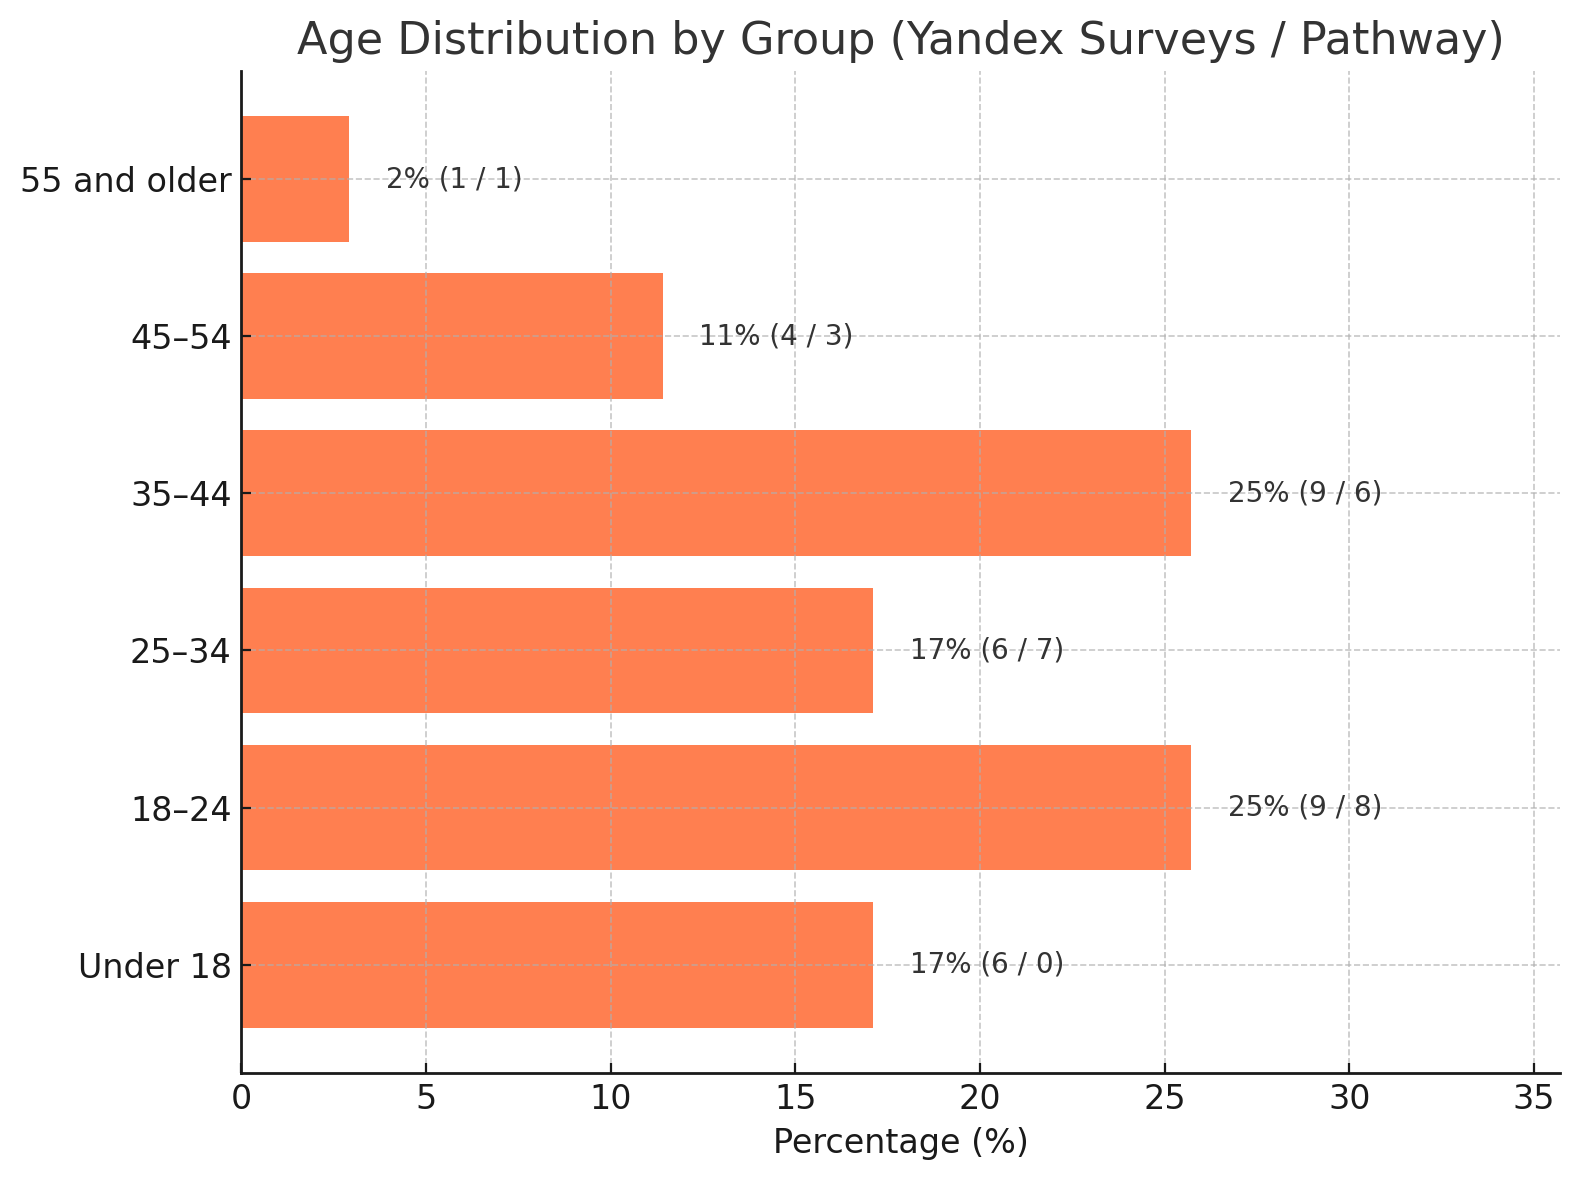
\includegraphics[width=1\linewidth]{figures/survey_age.png}
    \caption{Возрастное распределение участников}
    \label{fig:survey_age}
\end{figure}

Около 85\% участников (61 человек) на момент проведения опроса не использовали мобильные приложения для формирования привычек. Из них примерно 65\% никогда не пользовались такими приложениями, а 35\% использовали ранее, но перестали.

На вопрос о причинах удаления приложений ответили 17 человек. Наиболее часто упоминаемая причина, значительно выделяющаяся среди прочих, — ограниченный функционал в бесплатной версии.

Лишь 7 респондентов указали, какие приложения они используют в данный момент. Среди названных приложений — Finch, Google Sheets, MoveUp, Habit Tracker — Habit Diary, Forest, QuitZilla и Hizo.

На вопрос про срывы в формировании привычек ответили 65 респондентов. Наиболее часто участники называли эмоциональное и физическое истощение — чувство усталости, разбитости или измотанности (64,6\%). На втором месте — прокрастинация, когда выполнение привычки откладывается до последнего момента или вовсе игнорируется (43\%). Замыкает тройку лидеров занятость и нехватка времени (32,3\%).

\subsubsection{Основные выводы}

Из-за очень небольшого размера выборки нельзя с уверенностью определить, какие приложения наиболее популярны среди целевой аудитории, а также какие причины чаще всего приводят к отказу от их использования.

Тем не менее, результаты опроса позволяют сделать два вывода. 

Во-первых, приложениями для формирования привычек пользуется лишь небольшая часть респондентов. Это подтверждается и данными интервью: большинство участников либо вовсе не знали о таких приложениях, либо пробовали, но со временем отказались, либо не чувствуют уверенности в своих цифровых навыках, чтобы начать пользоваться этими приложениями.

Во-вторых, одной из самых частых причин срывов оказывается недостаточная простота действия — пользователи недостаточно упрощают свои привычки и в итоге отказываются от их выполнения из-за усталости. Этот вывод созвучен подходу Tiny Habits, согласно которому привычка должна быть настолько простой, чтобы её можно было выполнять практически без усилий. В рамках нашего приложения мы предложим пользователю сформулировать такую привычку, которую он сможет выполнять вне зависимости от уровня мотивации.

\subsubsection{Ограничения}

Основной недостаток проведённого опроса — низкая репрезентативность выборки, из-за чего полученные выводы нельзя напрямую распространить на всю целевую аудиторию. Однако важно, что участники были привлечены не через платформы с платными опросами, а через сообщества, посвящённые саморазвитию и формированию привычек — то есть максимально близкие к целевой аудитории. Кроме того, за участие не предлагалось денежное вознаграждение: вместо этого участники получали тематическую награду. Это снижало вероятность того, что опрос проходили только ради приза, и, скорее всего, способствовало более честным ответам. Таким образом, несмотря на ограниченность выборки, результаты опроса всё же отражают мнение людей, действительно заинтересованных в теме.

\subsection{Конкурентный анализ}\label{Competitor Analysis}

Последний вопрос, на который предстоит ответить в этом разделе, — что уже сделано для удовлетворения потребностей ЦА? Важно уточнить, что мы сосредоточим внимание исключительно на прямых конкурентах — мобильных приложениях для формирования привычек. Другие инструменты, в том числе упомянутые ранее по результатам интервью, в рамках этого анализа рассматриваться не будут.

Основных вопросов здесь три:

\begin{itemize}
    \item Каков функционал существующих мобильных приложений для формирования привычек?
    \item Как этот функционал согласуется с техниками изменения поведения, и какие из этих техник используются для поддержки формирования привычек?
    \item Насколько эти приложения удобны в использовании?
\end{itemize}

Ответ на первый вопрос позволяет понять, что в целом предлагают мобильные приложения для удовлетворения потребностей пользователей. Второй вопрос помогает оценить, насколько реализованный функционал может способствовать формированию привычек с точки зрения научных подходов к изменению поведения. Предполагается, что соответствие этим подходам повышает потенциальную эффективность приложений. Третий вопрос направлен на анализ удобства использования — важного фактора, влияющего на мотивацию и долгосрочное взаимодействие с приложением \cite{Biduski2020Assessing}.

\subsubsection{Процедура}

Систематический обзор был проведён в несколько этапов: поиск, скрининг, включение и анализ мобильных приложений, направленных на формирование новых привычек. Поиск осуществлялся вручную в апреле–мае 2025 года на следующих платформах: \textbf{Google Play}, \textbf{App Store}, \textbf{RuStore}, а также в \textbf{Google-поиске} (учитывались первые пять страниц поисковой выдачи).

В качестве поисковых запросов использовались ключевые слова на русском и английском языках. Англоязычные термины: \textit{“habit”}, \textit{“habit tracker”}, \textit{“best habit forming apps”}, \textit{“habit formation app”}. Русскоязычные: \textit{“трекер привычек”}, \textit{“привычки”}, \textit{“лучшие приложения для формирования привычек”}, \textit{“приложение для формирования привычек”}.

В обзор включались только те приложения, которые (1) были специально разработаны для формирования привычек, (2) поддерживают платформы Android или iOS, и (3) имеют не менее 100 установок. Исключались приложения, если они (1) не поддерживают русский или английский язык, (2) предназначены исключительно для детей, (3) фокусируются только на отслеживании настроения или времени, (4) отслеживают исключительно один тип привычек (например, чтение или подсчёт калорий), (5) доступны только на планшетах, (6) имеют рейтинг ниже 3{,}5 или менее трех отзывов, или (7) не обновлялись более двух лет до момента анализа. 

Первичный отбор проводился на основе описания приложения в магазине, после чего дополнительно учитывались рейтинг и количество отзывов. Далее для каждого включённого приложения осуществлялся сбор и анализ следующих данных: функциональность, используемые техники изменения поведения (Behavior Change Techniques, BCT) согласно существующей таксономии \cite{michie_2008_bct}, наличие элементов формирования привычек.

Также проводилась эвристическая оценка интерфейса по десяти принципам юзабилити Нильсона. Каждый принцип оценивался по 10-балльной шкале, где:

\begin{itemize}
    \item 1–2 — очень плохо: эвристика практически не реализована, вызывает серьёзные затруднения;
    \item 3–4 — плохо: реализация неудовлетворительная, имеются значимые проблемы;
    \item 5–6 — удовлетворительно: эвристика реализована частично, с огрехами;
    \item 7–8 — хорошо: реализация близка к полной, имеются незначительные недостатки;
    \item 9–10 — отлично: эвристика реализована полностью, пользовательский опыт положительный.
\end{itemize}

Полученные данные обобщены в таблице и проанализированы с использованием описательных методов. Полный перечень проанализированных приложений, включая их характеристики, эвристические оценки и используемые техники изменения поведения, представлен в электронной таблице: \href{https://docs.google.com/spreadsheets/d/1RScNqPcjewJ4yKeazq6BL-yURvEvElnoeXhkra210Ag/edit?usp=sharing}{ссылка на данные}.

\subsubsection{Результаты}

Первичный поиск выдал 601 приложение. После удаления дубликатов осталось 592 уникальных приложения. После применения критериев включения и исключения в анализ было включено 66 приложений.

\textit{Функциональность}. Анализ приложений показал, что большинство из них предлагают схожий базовый набор функций. Почти во всех приложениях (95\%) можно добавить собственную привычку. Почти 80\% приложений предлагают напоминания. Третья по распространённости функция — статистика и отслеживание прогресса (70\%). Около 40\% приложений включают календарь и отслеживание «стрика» — серии дней с выполненной привычкой. Примерно треть приложений позволяют выбирать тему оформления или добавлять заметки к привычке. Готовые шаблоны привычек и возможность выбора периодичности (день, неделя и т.д.) встречаются примерно в каждом третьем приложении. У 17\% приложений имеется функция выбора типа привычки (например, вредной или полезной). На рисунке \ref{fig:top_features} показано 10 наиболее распространенных функций в рассмотренных приложениях.
 
\begin{figure}[]
\centering
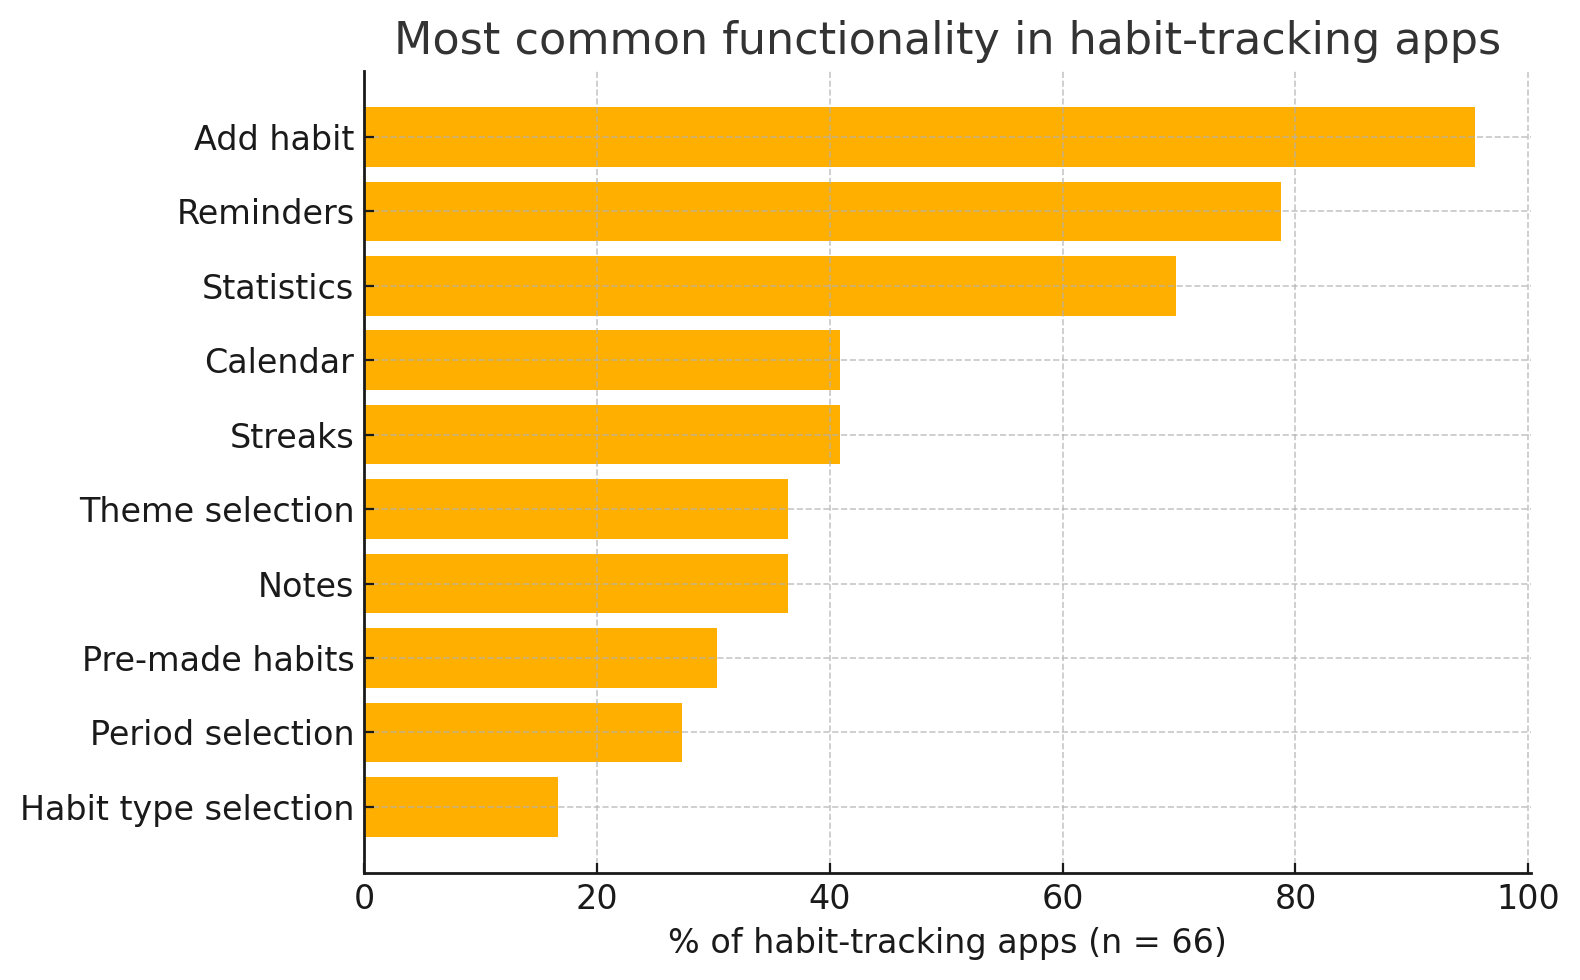
\includegraphics[width=0.8\textwidth]{figures/top_features_chart.png}
\caption{Топ-10 самых распространённых функций в трекерах привычек (n=66)}
\label{fig:top_features}
\end{figure}

Реже всего среди рассмотренных приложений встречается функция расчёта «силы» привычки — она реализована лишь в одном случае, в Loop Habit Tracker. Ещё менее распространены функции на основе искусственного интеллекта: поддержку ИИ предлагают только два приложения. RoutineFlow использует ИИ для генерации персонализированных рекомендаций, а Wipepp предлагает чат с виртуальным ассистентом.

Особую категорию составляют приложения, полностью построенные на геймификации. К ним относятся Habitica и Habit Hunter: RPG Goal Tracker. В Habitica пользователь создаёт собственного персонажа, который развивается по мере выполнения привычек и задач. За успешное выполнение целей начисляются очки опыта и внутриигровая валюта, которую можно тратить на экипировку или награды. Пропуск задач, напротив, снижает здоровье персонажа. Таким образом, формирование привычек становится частью игрового процесса, где каждое действие влияет на прогресс героя. 

Habit Hunter развивает геймификацию в формате приключенческой RPG. Здесь пользователь перемещается по карте, сражается с монстрами и выполняет квесты, связанные с его реальными делами и привычками. Каждое выполненное задание помогает продвинуться по сюжету и открывает новые игровые возможности. 

\textit{Поддержка формирования привычек}. Наиболее широко распространёнными техниками изменения поведения (behavior change techniques, BCTs) в анализируемых приложениях стали: подсказки и напоминания (Prompts/Cues), обратная связь о поведении (Feedback on Behavior), самонаблюдение (Self-Monitoring) и постановка целей (Goal Setting). Эти методы присутствуют практически во всех приложениях.

Подсказки и напоминания почти повсеместно реализованы в виде настраиваемых push-уведомлений, помогающих пользователю не забывать о целевом поведении. Обратная связь о поведении чаще всего представлена визуализацией прогресса (например, графики или календарные отметки), а также в некоторых случаях — элементами социальной поддержки, как в MyRoutine или Habitica. Самонаблюдение реализуется через систему отметок о выполнении привычек, позволяя пользователю отслеживать свою активность. Постановка целей (Goal Setting), как правило, представлена в форме создания новой привычки с возможностью задать её название, описание, частоту и другие параметры.

Однако есть небольшая группа стратегий, которые встречаются крайне редко. Лишь одно приложение Habitica содержит такие приёмы, как «incentive (outcome)» (обещание внешней награды за достижение результата), «social incentive» (поощрение через общественное признание), «self-incentive» (самопоощрение), «social comparison» (сравнение с другими пользователями) и только Atoms использует «review outcome goal» (рефлексия достигнутой цели). Ещё реже, но всё же чуть чаще (около 3\%) реализуется стратегия «punishment» – применение штрафа или лишения вознаграждения при невыполнении задачи.

Следующая по редкости группа включает «commitment», «social support» и «action planning» (детальная проработка плана действий) – каждую из них использует не более 4-6\% приложений. Наконец, техника «instruction on how to perform a behavior» встречается в 7,6\% случаев.

Сопоставление функционала с ключевыми факторами формирования привычек демонстрирует явный перекос в сторону цифровых напоминаний и самоконтроля при почти полном отсутствии средств, помогающих встроить новое поведение в контекст повседневной жизни. Только 3 приложения (около 5\%) содержат явную поддержку «implementation intentions» – формулировок вида «Когда X, то делаю Y». В двух приложениях — Fabulous и Atoms — присутствует якорение (привязка поведения к уже существующей рутине) в явном виде. Позитивное подкрепление реализуется в виде виртуальных наград лишь в каждом пятом случае.

Наиболее полно научным принципам формирования привычек соответствует приложение Atoms — во многом благодаря тому, что в его создании участвовал Дж. Клир, автор популярной концепции «атомных привычек». Несмотря на то, что в Atoms реализовано меньше техник изменения поведения, чем в Fabulous и Habitica, эти техники встроены в целостную и логично выстроенную систему. Однако важным недостатком приложения остаются жёсткие ограничения: даже в платной версии нельзя отслеживать более трёх привычек одновременно. Это может быть оправдано с точки зрения эффективности формирования привычек, но при этом пользователю не хватает гибкости — невозможно, например, заранее сохранить дополнительные привычки, чтобы вернуться к ним позже.

\textit{Удобство использования}. Средняя интегральная оценка составила 8,4 ± 1,9 балла, что соответствует уровню «хорошо». Большинство измерений (около 60\%) попадают в диапазон «отлично», ещё четверть (около 24\%) — в категорию «хорошо». Значения «плохо» и «очень плохо» встречались редко (меньше 5\% и < 1\% соответственно), что говорит о в целом высоком качестве юзабилити рассматриваемых интерфейсов. 

Наивысшие средние баллы получили эвристики «Справка и документация» (Q10 = 9,5), «Помощь в распознавании и исправлении ошибок» (Q9 = 9,5) и «Предотвращение ошибок» (Q5 = 9,3). Пользователи легко находят подсказки (а часто им подсказки вовсе оказываются не нужны), получают внятные сообщения об ошибках и редко допускают критические промахи благодаря предусмотренным ограничениям и подтверждениям. Это создаёт ощущение надёжности и снижает когнитивную нагрузку при работе с приложениями.

Самыми «слабыми» остались «Гибкость и эффективность использования» (Q7 = 7,5) и «Согласованность и стандарты» (Q4 = 7,5). В обзоре встречались приложения, где продвинутые функции скрыты слишком глубоко, а паттерны навигации отличаются от принятых в мобильных ОС. Часть сервисов реализует уникальные жесты или терминологию, что затрудняет быстрое освоение. Хотя средние оценки всё ещё находятся в зоне «хорошо», именно здесь наблюдался наибольший разброс: от единичных «очень плохо» (1–2 балла) до максимальных показателей, что указывает на неравномерность качества внутри выборки. 

По результатам эвристической оценки наивысший совокупный балл (9,8 из 10) показали три приложения — Streaks (iOS), Habit Tracker — Habit Diary (Android) и Hizo (Android, iOS). Каждое из них стабильно набирало от 9 до 10 баллов практически по всем десяти эвристикам юзабилити Нильсона. Благодаря такому равномерно высокому уровню реализации эвристик они заняли первые места в рейтинге и могут служить эталоном удобства использования в проанализированной выборке мобильных трекеров привычек.

\subsubsection{Основные выводы}

Результаты проведённого анализа подтверждают ключевые наблюдения, ранее описанные в работе Stawarz et al. (2015): большинство приложений сосредоточены на функциях напоминания и самонаблюдения, тогда как поддержка более глубоких поведенческих стратегий и контекстной интеграции привычек остаётся ограниченной. Подобно результатам исследования Stawarz, выявлено преобладание поверхностных функций — таких как добавление привычек, напоминания и трекинг — при недостаточной реализации методов, способствующих устойчивому формированию поведения, включая implementation intentions, планирование действий (action planning) и использование контекстуальных сигналов (contextual cues) \cite{stawarz_beyond_2015}.

Среди всех рассмотренных решений наибольшую проработанность с точки зрения техники формирования привычек и качества пользовательского опыта продемонстрировало приложение Atoms, созданное при участии Дж. Клира. Несмотря на ограниченное количество реализованных методик, Atoms предлагает целостную поведенческую модель, в которой каждая техника встроена в логичную стратегию изменения поведения. В частности, в приложении представлены такие элементы, как якорение (anchoring), переоценка целевых установок (review of outcome goals) и implementation intentions. Приложение также отличается высоким уровнем удобства использования. Однако жёсткое ограничение на количество одновременно отслеживаемых привычек снижает его гибкость и универсальность, особенно для более опытных пользователей.

Следует также отметить, что ни одно из проанализированных приложений не реализует методику Tiny Habits в её полном виде. Хотя отдельные техники (например, якорение) перекликаются с её принципами, целостного и структурированного подхода, соответствующего данной методике, не представлено.

\subsubsection{Ограничения}

Конкурентный анализ ограничен рядом методологических допущений. Во-первых, поиск выполнялся вручную и охватывал лишь апрель-май 2025 г.; при этом анализировались только первые пять страниц Google Search и витрины трёх магазинов (Google Play, App Store, RuStore), поэтому приложения, продвигаемые слабее по SEO либо распространяемые через альтернативные каналы (например, Huawei AppGallery или веб-версии), могли быть пропущены. Во-вторых, использовался фиксированный набор ключевых слов («habit», «habit tracker», «трекер привычек» и др.), который не покрывает близкие синонимы вроде «routine planner» или «daily tracker», ограничивая полноту выборки. В-третьих, жёсткие критерии включения ($\geq100$ установок, рейтинг $\geq3{,}5$, обновление не позднее двух лет, поддержка только русского или английского интерфейса) отсекли молодые проекты и локальные продукты на других языках, сместив выборку в сторону зрелых массовых решений. В-четвёртых, функциональность платных приложений и закрытых модулей freemium-моделей не тестировалась напрямую; выводы о них основаны на косвенных данных (видеообзоры, отзывы, описания разработчиков), что может приводить к неполному или искажённому представлению о реальных возможностях. Наконец, кодирование Behavior Change Techniques и эвристическая оценка юзабилити проводились одним исследователем без двойного слепого рецензирования и расчёта Cohen's $\kappa$, что повышает риск субъективности и снижает воспроизводимость результатов.

\subsection{Итоги раздела}\label{Requirements}

Раздел «Контекст и потребности» дал возможность глубже узнать о целевой аудитории, ее потребностях и степени их удовлетворения. 

Аудитория оказалась разной — как по возрасту и профессии, так и по опыту взаимодействия с цифровыми инструментами. Людей объединяет стремление к саморазвитию: они хотят становиться организованнее, здоровее, увереннее в себе. При этом мотивация и ожидания у всех разные — кто-то настроен на постепенные изменения, кто-то ждёт ощутимого результата уже через пару недель.

Основные потребности пользователей связаны с простотой. Люди хотят, чтобы привычку было легко выполнять и легко отслеживать — без лишних усилий и сложных интерфейсов. Важно, чтобы сама привычка воспринималась как осмысленное действие, а не как «надо просто потому, что надо». Поэтому многим важно сначала понять, действительно ли привычка приближает их к личной цели. Пользователи также хотят видеть прогресс, но без давления: если что-то не получилось, это не должно вызывать чувство вины или обесценивать предыдущие успехи. Особое значение имеет гибкость — возможность задавать нерегулярные привычки и управлять частотой так, как удобно. Ещё одна важная тема — устойчивость: привычка должна «держаться» даже в условиях усталости, занятости или временного сбоя в расписании.

Опрос подтвердил, что наиболее частыми причинами срывов становятся усталость, эмоциональное выгорание и откладывание действия «на потом». Эти факторы особенно критичны, когда сама привычка слишком сложная или требует много энергии. Это согласуется с подходом Tiny Habits, согласно которому даже небольшое и простое действие может лечь в основу устойчивого поведения. Однако опрос и интервью также показали, что для части пользователей важно видеть результат достаточно быстро — иначе мотивация снижается. Это означает, что приложение должно не только упрощать действия, но и помогать пользователю почувствовать пользу от них как можно раньше.

В ходе конкурентного анализа стало ясно, что большинство существующих приложений для формирования привычек ограничиваются базовыми функциями: добавление задач, напоминания, календарь и статистика. Более глубокие поведенческие техники, такие как якорение привычек или планирование действий, реализованы редко. Даже те приложения, которые выглядят продуманными с точки зрения интерфейса, не всегда обеспечивают поведенчески эффективную поддержку. Ни одно из проанализированных решений не использует метод Tiny Habits в своей основе.

Таким образом, можно выделить следующие требования к приложению:

\begin{itemize}
    \item \textbf{Простота взаимодействия.} Пользователю должно быть понятно, как пользоваться приложением с первых минут. Любое действие (например, отметка привычки) не должно требовать значительных усилий или времени.

    \item \textbf{Осмысленность действия.} Приложение должно помогать человеку понять, зачем ему конкретная привычка и как она связана с его личными целями. Поведение не должно быть формальным — только ради галочки.

    \item \textbf{Гибкость в настройке.} Пользователь должен иметь возможность адаптировать ритм и формат выполнения привычек под свой график, включая нерегулярные или редкие действия.

    \item \textbf{Поддержка в условиях снижения мотивации.} Интерфейс и сценарии использования не должны требовать высокого уровня энергии или настроя — привычки должны оставаться выполнимыми даже в сложные дни.

    \item \textbf{Устойчивость привычек.} Приложение должно поддерживать пользователя в случае пропусков, не обнулять прогресс и помогать вернуться к привычке после перерывов (например, отпуска или болезни).

    \item \textbf{Позитивная обратная связь.} Важно, чтобы пользователь регулярно получал подтверждение, что его усилия имеют значение — это может быть визуальный прогресс, мягкое поощрение или напоминание о достигнутом.

    \item \textbf{Минимальное когнитивное и эмоциональное напряжение.} Приложение не должно нагружать пользователя избыточной информацией, сложными настройками или тревожными уведомлениями.

    \item \textbf{Уважение к приватности и автономии.} Пользователь должен чувствовать, что контролирует свои данные и взаимодействие с приложением. Приложение не должно вызывать ощущения внешнего контроля.

    \item \textbf{Доступность для пользователей с разным уровнем цифровых навыков.} Интерфейс и инструкции должны быть понятны как опытным пользователям, так и тем, кто неуверенно чувствует себя в цифровой среде.

    \item \textbf{Поддержка формирования привычки в повседневном контексте.} Поведение должно быть встроено в существующие рутинные действия, а не восприниматься как отдельное, требующее специального времени.

\end{itemize}

Сформулированные требования лягут в основу проектирования мобильного приложения «Habiteer». О процессе его разработки — в следующих разделах.

\newpage

\section{Разработка логики приложения: Телеграм-бот}\label{Development}

\subsection{Обзор раздела}

Поскольку мобильное приложение разрабатывается на основе метода Tiny Habits, оно должно учитывать не только требования, изложенные в конце первого раздела, но и особенности самого метода. Алгоритм Tiny Habits ранее был показан на рис. \ref{fig:pic2}, но теперь имеет смысл рассмотреть его более подробно.

Процесс формирования полезных привычек по этому методу включает следующие шаги:

\begin{enumerate}
    \item \label{th:aspiration} \textbf{Прояснить стремление}. Под стремлением понимается нечто менее конкретное, чем цель, — скорее общее желание или желаемый результат. Например, стремлениями могут быть: «питаться правильно», «стать продуктивнее», «выучить английский». Определить стремление — значит задать себе вопрос: «Действительно ли я этого хочу? Или это средство для достижения чего-то другого?». Например, человек может думать, что хочет «питаться правильно», но если за этим стоит желание похудеть, то истинным стремлением является «сбросить вес».
    \item \label{th:beh_explore} \textbf{Исследовать варианты поведения}. После того как стремление определено, происходит мозговой штурм конкретных действий, которые могут привести к реализации стремления.  Например, если стремление — «сбросить вес», возможные действия могут включать: «не есть после 20:00», «добавить овощи к каждому приёму пищи», «ходить по 10 тысяч шагов в день». На этом этапе важно не ограничивать себя критикой — задача состоит в том, чтобы собрать как можно больше идей. Среди них могут быть как регулярные действия, так и одноразовые мероприятия, а также привычки, от которых стоит отказаться.
    \item \label{th:beh_crispify} \textbf{Уточнить варианты поведения}.  Далее необходимо убедиться, что предложенные варианты являются достаточно конкретными. Например, «заниматься спортом» — слишком общее поведение, тогда как «делать 10 отжиманий после пробуждения» — конкретное и измеримое. Чем яснее и точнее сформулировано поведение, тем легче будет его реализовать.
    \item \label{th:beh_eval} \textbf{Выбрать подходящие действия}. После генерации и уточнения вариантов поведения наступает этап их отбора. Для этого применяется метод Focus Mapping, который позволяет одновременно учитывать два критерия: предполагаемую эффективность действия (насколько оно приближает к стремлению) и его выполнимость (насколько легко его реализовать в повседневной жизни). Все варианты поведения размещаются на условной плоскости, где по горизонтали откладывается простота выполнения, а по вертикали — польза действия. В результате визуально выделяется так называемая «золотая зона» — это те действия, которые и полезны, и легко выполнимы. Именно с них рекомендуется начинать, поскольку они создают наилучшие условия для формирования устойчивой привычки.
    \item \label{th:simlpify} \textbf{Упростить поведение}. Преобразовать выбранное действие в максимально простой и короткий вариант, который можно выполнять без усилий и предварительной подготовки. Для этого сначала рекомендуется задать себе вопрос: «Что делает это поведение сложным?» и проанализировать поведение с точки зрения цепочки способности (ability chain), включающей такие факторы, как время, деньги, физические усилия, ментальные усилия и соответствие существующим привычкам. Затем следует задать второй вопрос: «Как я могу сделать это поведение легче?». Для этого можно применить один или несколько из трёх способов: развить навыки (требуется более высокая мотивация), получить недостающие ресурсы, либо упростить поведение. Упрощение поведения может принимать две формы: starter step — начать с самого первого шага (например, «достать коврик для йоги» вместо «заниматься йогой»), или scaling back — выполнить действие в сокращённом варианте (например, «сделать одно отжимание» вместо запланированных десяти).
    \item \label{th:trigger} \textbf{Найти подходящую «подсказку» (триггер)}.  Подобрать уже существующее действие или событие в повседневной жизни, которое будет служить напоминанием о новой привычке. Такая «подсказка» должна быть стабильной, легко узнаваемой и регулярно повторяющейся. Чаще всего в качестве триггера используют рутинные действия, например: «после того как почищу зубы», «после того как включу чайник», «когда сяду за рабочий стол». Новое поведение привязывается к этому действию по формуле: «После того как [триггер], я [новое поведение]». Чтобы такая связка работала надёжно, рекомендуется учитывать три критерия: поведение и триггер должны происходить в одном и том же месте (соответствие физическому расположению), с одинаковой частотой (совпадение по регулярности), а также быть логически связаны по смыслу или назначению (тематическое соответствие).
    \item \label{th:repeat} \textbf{Отрепетировать привычку}. После того как привычка определена, упрощена и привязана к подходящему триггеру, рекомендуется несколько раз отрепетировать её выполнение в реальных условиях. Это помогает укрепить связь между триггером и действием, а также снижает психологический барьер перед началом. После каждого выполнения привычки следует сразу же отпраздновать успех — с помощью короткой позитивной реакции: улыбки, жеста, фразы вроде «Отлично!» или внутреннего ощущения гордости. Такой эмоциональный отклик усиливает положительное восприятие действия и способствует его закреплению на уровне автоматического поведения.
    \item \label{th:implement} \textbf{Внедрять привычку в жизнь}.  На этом этапе привычка начинает регулярно применяться в реальных условиях. Если выполнение забывается, полезно снова отрепетировать поведение, чтобы восстановить связь между триггером и действием. Если забывания продолжаются, возможно, выбранный триггер не подходит — в этом случае его стоит заменить на более надёжный. Если же привычка оказывается слишком сложной для регулярного выполнения, её следует дополнительно упростить, например, сократив объём действия или вернувшись к начальному шагу.
\end{enumerate}

Эти шаги станут основой функциональной логики мобильного приложения, однако автор оставляет за собой возможность адаптировать и модифицировать их структуру. Такие изменения будут осуществляться в зависимости от потребностей целевой аудитории и требований, изложенных в первом разделе, с обязательным сохранением ключевых принципов метода Tiny Habits. 

Приложение «Habiteer» можно рассматривать с двух сторон: логики и пользовательского интерфейса. Под интерфейсом понимается визуальное и интерактивное представление элементов приложения, а под логикой — внутренняя организация компонентов и сценариев, лежащих в основе пользовательского опыта. При этом логика определяет интерфейс: то, как устроен путь пользователя внутри приложения, напрямую влияет на то, как этот путь будет представлен визуально. Поэтому в этом разделе основное внимание уделяется именно логике.

Метод Tiny Habits, описанный выше, служит основой для проектирования этой логики. Задача состоит не просто в том, чтобы точно передать шаги метода, но и в том, чтобы сделать их понятными, простыми и естественными для пользователя. Отсюда возникают два ключевых вопроса раздела:

\begin{itemize}
    \item Какая должна быть логика у приложения?
    \item Насколько предложенная логика может обеспечить более эффективное формирование привычек, а также насколько она удобна в использовании по сравнению с лучшими существующими аналогами?
\end{itemize}

Чтобы это проверить, была создана тестовая версия в виде Telegram-бота. Такой формат позволяет быстро и с минимальными затратами протестировать ключевые сценарии, не разрабатывая сразу полноценное мобильное приложение.

\subsection{Тестирование бумажного прототипа}

Разработка даже простой версии Телеграм-бота требует времени и ресурсов. Бумажный прототип помогает значительно сократить затраты на этом этапе за счёт предварительной проработки интерфейса и логики взаимодействия. Он позволяет:

\begin{enumerate}
\item Упростить процесс создания чат-бота, так как структура взаимодействия с пользователем уже выстроена;
\item Оценить понятность и удобство интерфейса до начала программной реализации;
\item Собрать обратную связь и выявить потенциальные ошибки или неочевидные моменты в логике.
\end{enumerate}

Цель тестирования бумажного прототипа — понять, насколько предложенная идея сервиса интуитивно ясна, привлекательна и практически реализуема с точки зрения конечного пользователя. В частности, важно:

\begin{itemize}
\item Оценить понятность концепции сервиса и его ценности;
\item Собрать первое впечатление пользователей о предполагаемой логике работы;
\item Выявить проблемные места в интерфейсе бота и структуре взаимодействия;
\item Уточнить ожидания пользователей.
\end{itemize}

\subsubsection{Дизайн бумажного прототипа}

Для создания бумажного прототипа были использованы карточки размером 115 × 65 мм, вырезанные из листов формата A4. На лицевой стороне каждой карточки изображён один экран интерфейса с основными элементами управления: текстами, кнопками, полями ввода и другими компонентами. На оборотной стороне указан уникальный идентификационный номер, позволяющий быстро ориентироваться в структуре прототипа. Всего было подготовлено 45 таких карточек. Пример можно видеть на рисунке \ref{fig:bot_cards}.

\begin{figure}[]
\centering
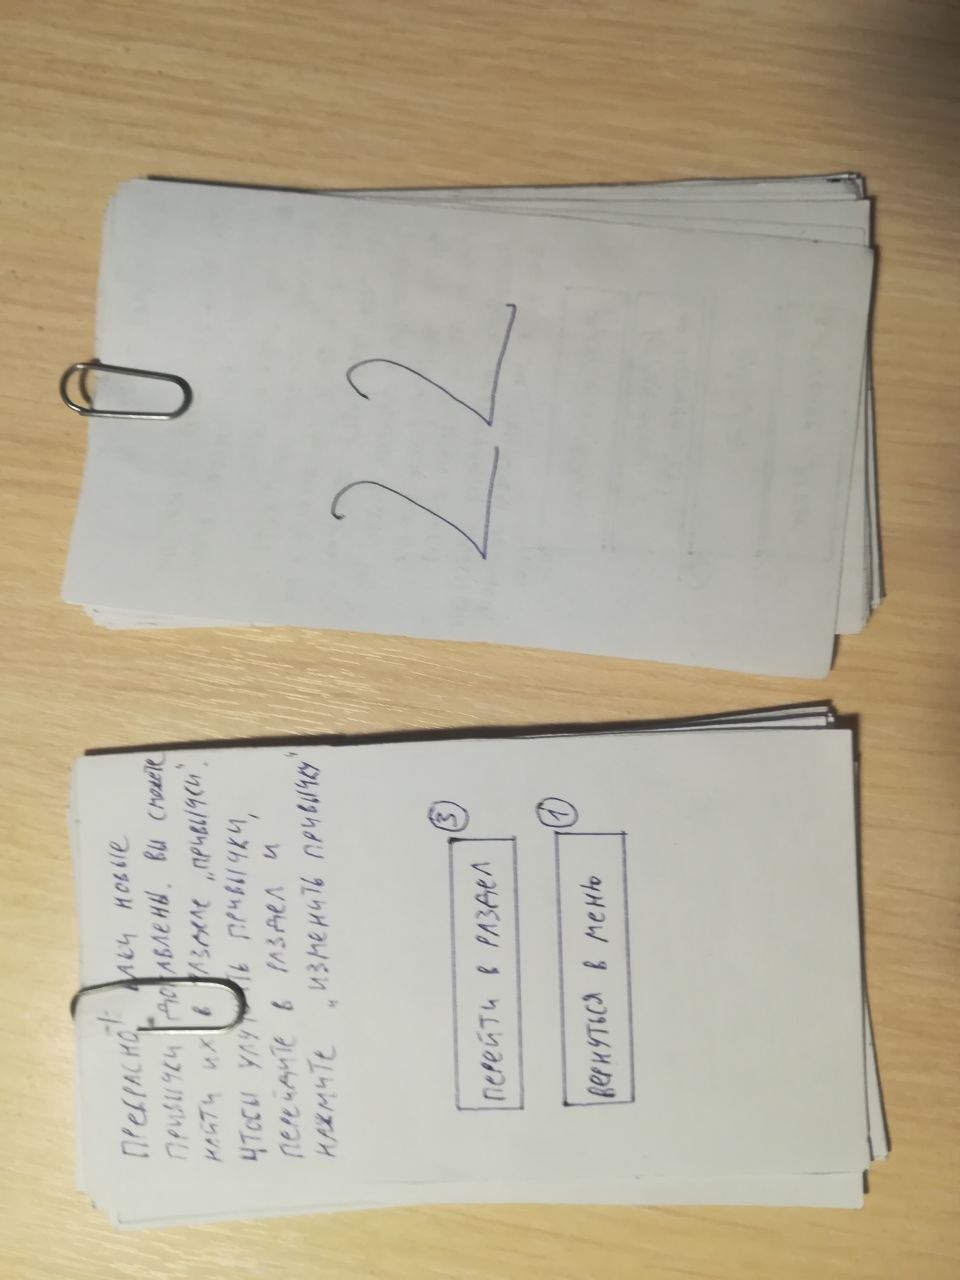
\includegraphics[width=0.7\textwidth, angle=270]{figures/bot_cards.jpg}
\caption{Карточки, использованные для бумажного прототипирования интерфейса}
\label{fig:bot_cards}
\end{figure}

Бумажный прототип состоит из следующих основных функций:

\begin{itemize}
    \item \textbf{Добавить привычку}. При нажатии на соответствующую «кнопку» пользователю предлагается ввести новую привычку. При этом отображается подсказка: необходимо вводить конкретное поведение, а не общее стремление.
    \item \textbf{Изменить данные о привычке}. Пользователь может изменить название привычки, выбрать её тип и начать отслеживание. Под «отслеживанием» подразумевается то, что привычку можно будет впоследствии отмечать с помощью отчетов, которые будут приходить в указанное пользователем время. Чтобы включить отслеживание, пользователь выбирает тип триггера — «другое поведение» или «уведомление в телефоне». Предпочтительным считается первый вариант. Если выбран триггер в виде уведомления, то настраиваются их периодичность и время. Если выбран триггер-поведение, пользователь должен описать действие, после которого он будет выполнять привычку. Далее предлагается отрепетировать привычку 7–10 раз после триггера-поведения. Если на это нет времени или это невозможно, пользователь выбирает соответствующие опции, нажав на кнопку «нет возможности». Независимо от того, какой тип триггера был выбран, если пользователь не выбрал вариант с напоминанием о репетиции, ему в любом случае предлагается настроить время получения отчёта для этой привычки.
    \item \textbf{Подобрать привычку}. Пользователю предлагается список из десяти готовых стремлений: например, правильно питаться, лучше спать, лучше справляться со стрессом и т.д. Он выбирает одно из них, и ему предлагаются готовые привычки, из которых он может выбрать 1-3. Если ни одно готовое стремление не подходит, ему предлагается написать собственное стремление, а затем уточнить: действительно ли он этого хочет или ему это нужно для достижения другого стремления? В первом случае, он переходит к этапу мозгового штурма вариантов поведения, а во втором, он возвращается к стремлению, которое ему придется переписать. Далее пользователь придумывает как минимум 5 вариантов поведения и оценивает их с точки зрения эффективности и выполнимости. Наконец, ему предлагаются наиболее подходящие привычки. Он может их оставить, выбрав опцию «То, что нужно!» или вернуться на предыдущие шаги алгоритма, в зависимости от того, что он хочет — изменить приоритеты или добавить новые варианты поведения.
    \item \textbf{Статистика}. Отображаются текущий и лучший стрик по всем привычкам.
    \item \textbf{Настройки}. Пользователь может включить или отключить мотивационные сообщения, задать время отчётов, отправить отзыв или удалить свои данные.
\end{itemize}

\begin{figure}[]
\centering
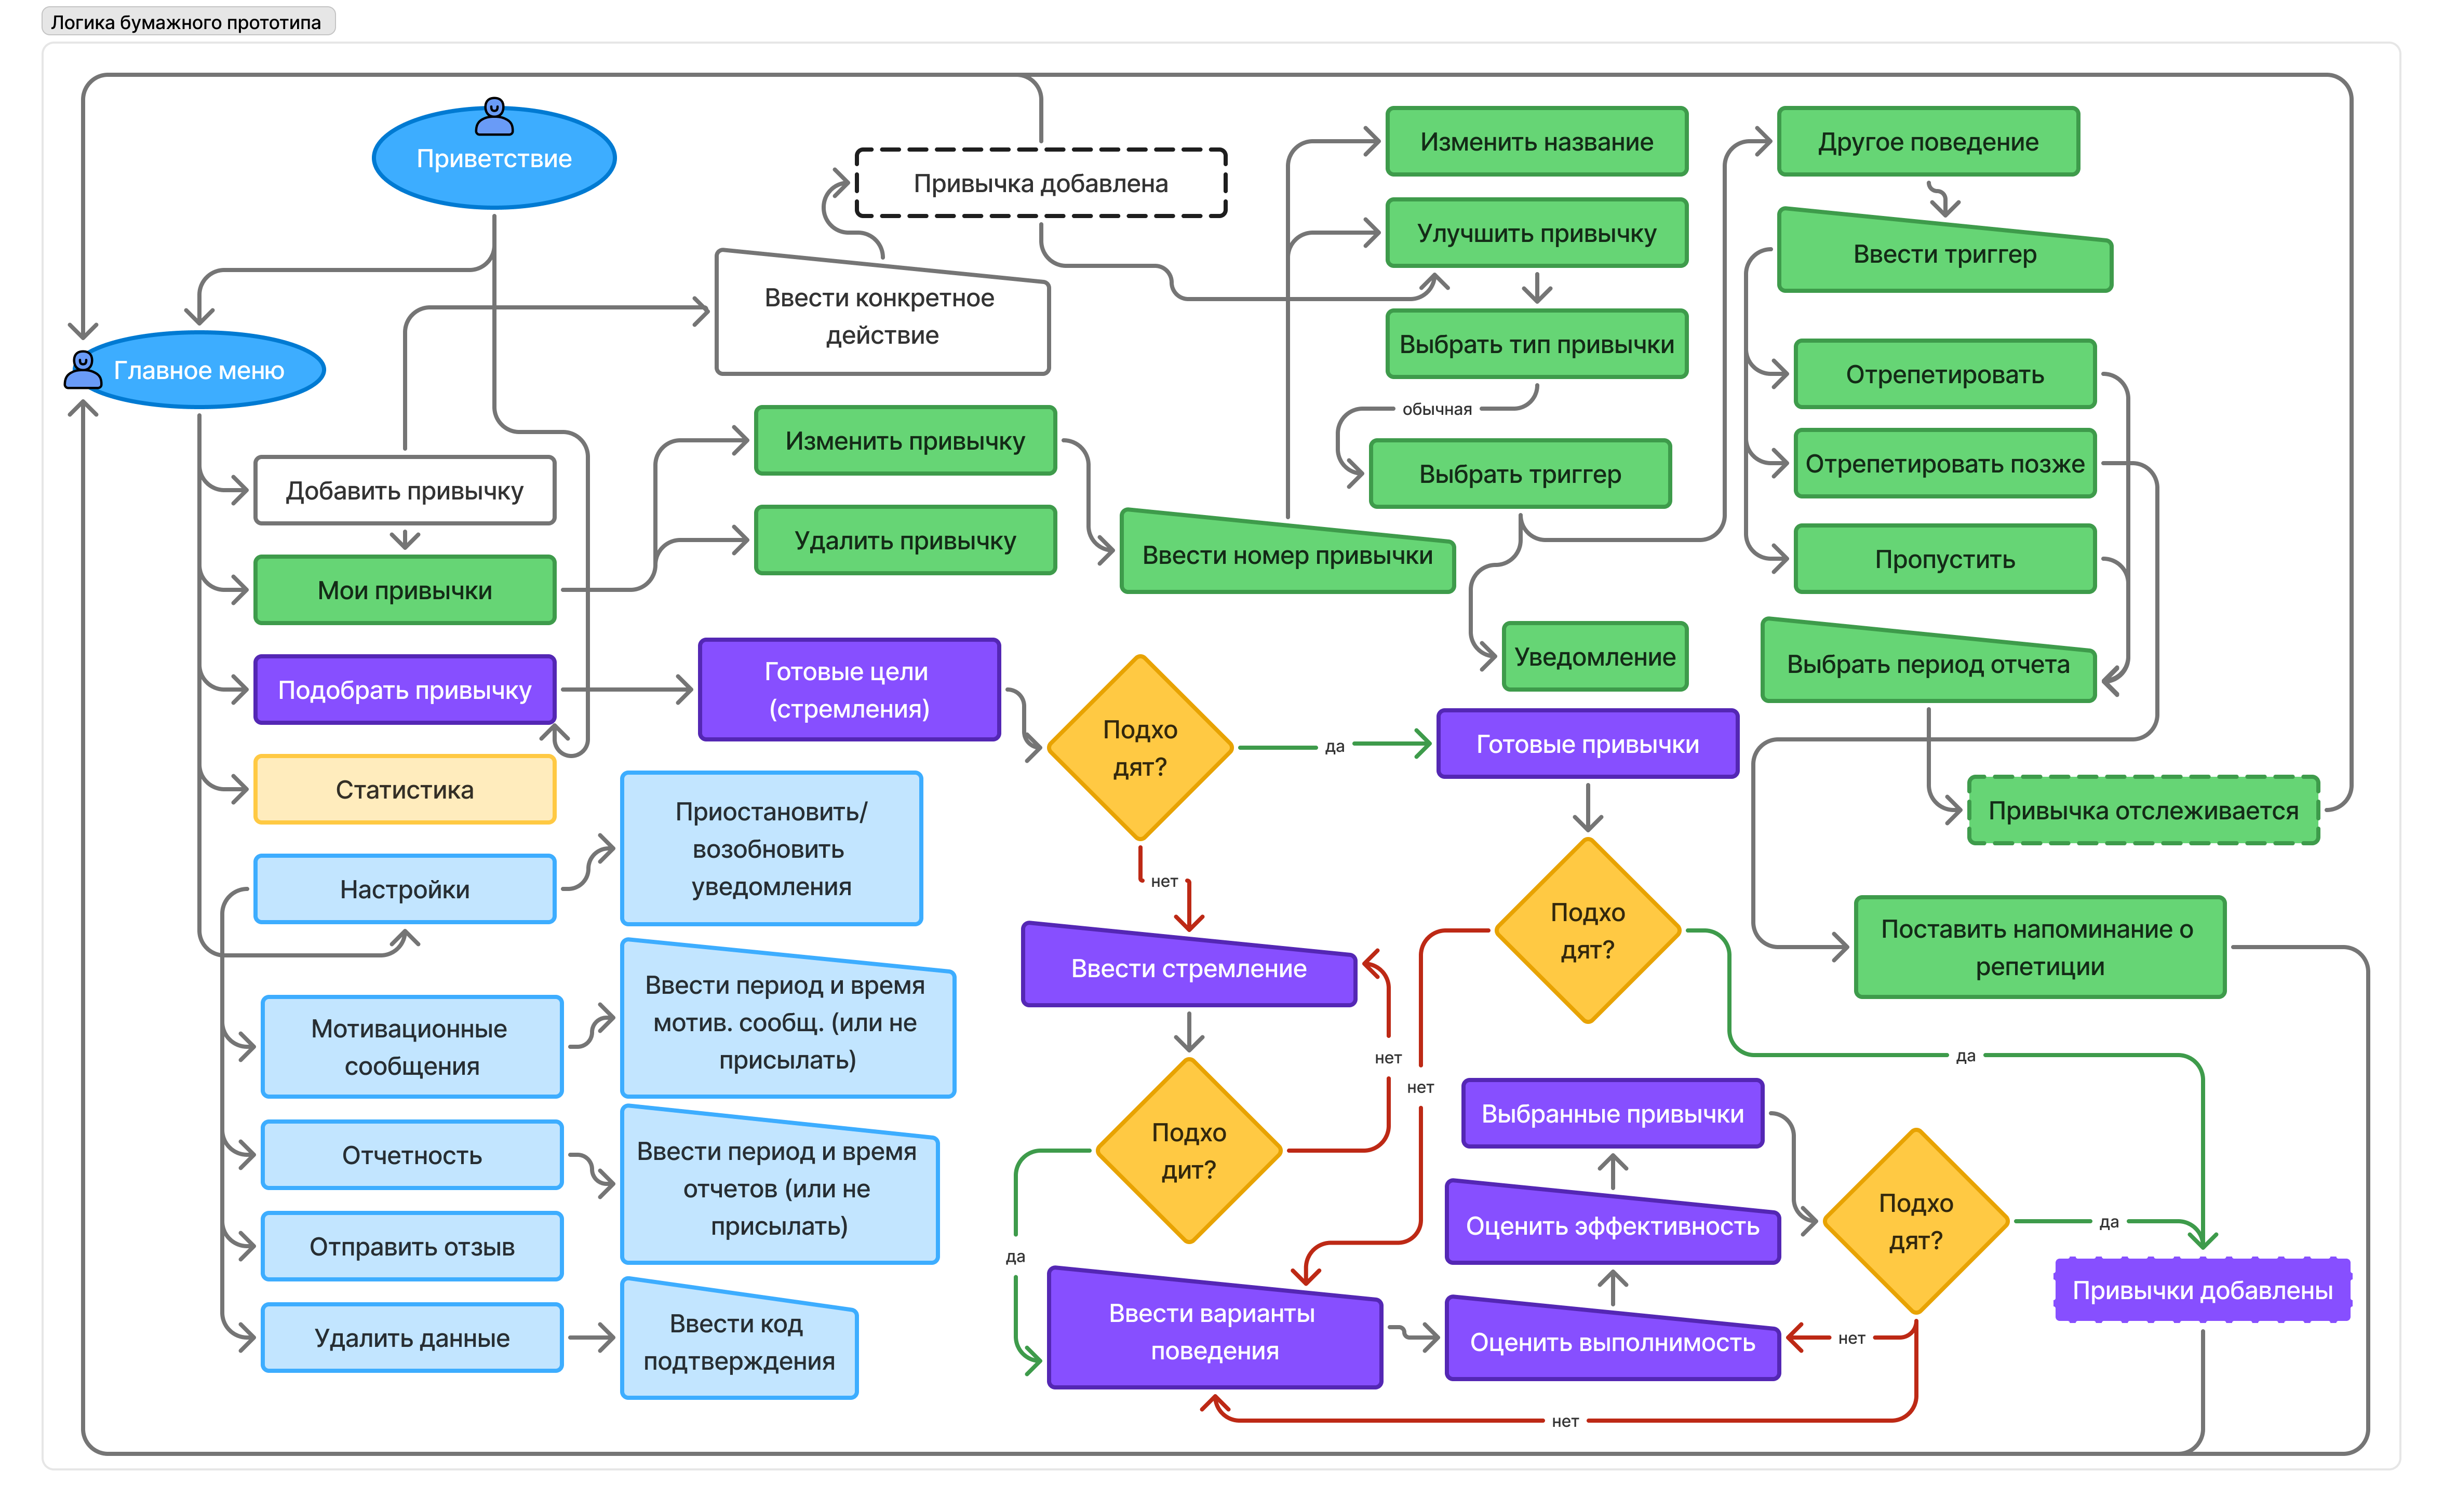
\includegraphics[width=1.1\textwidth]{figures/paper_prototype_logic.png}
\caption{Логика бумажного прототипа}
\label{fig:paper_bot_logic}
\end{figure}

Логика работы прототипа представлена на рисунке \ref{fig:paper_bot_logic}. 

\subsubsection{Процедура и задачи}

В ходе тестирования бумажного прототипа автор стремился ответить на следующие исследовательские вопросы:

\begin{itemize}
\item Насколько легко участникам было добавить новую привычку?
\item Насколько понятным оказался алгоритм подбора привычек?
\item Понимали ли участники, как работает механизм улучшения привычек?
\item Корректно ли они вводили названия привычек? Осознавали ли, что привычка должна быть конкретным поведением?
\item Насколько понятными были формулировки и пояснения, представленные в интерфейсе?
\item Что участники ожидали увидеть в разделе «Статистика»?
\item Какое представление у них сформировалось о чат-боте на основе предложенного прототипа? Какие мнения они высказывали о нём?
\end{itemize}

Тестирование проводилось в формате индивидуальных модерируемых сессий продолжительностью 30–45 минут. Взаимодействие с интерфейсом моделировалось с помощью «переходов» между карточками: возле нарисованных кнопок указывались номера карточек, которые следовало открыть после «нажатия». Все карточки, кроме текущей, оставались закрытыми.

Сессия начиналась с карточки, помеченной как «/start». Взаимодействие сопровождалось имитацией системных реакций — подсчётов, ответов чат-бота и других действий, которые в реальном Телеграм-боте выполнялись бы автоматически. Эти элементы интерактивности воспроизводились модератором по заранее подготовленному сценарию с использованием метода Wizard-of-Oz.

В рамках исследования собирались исключительно качественные данные. Участники проговаривали свои действия вслух, следуя протоколу think-aloud. После выполнения сценария проводилось короткое follow-up интервью, в ходе которого участники делились общими впечатлениями от взаимодействия с прототипом и описывали наиболее затруднительные моменты. Модератор уточнял наблюдения и, при необходимости, задавал дополнительные вопросы.

В рамках тестирования участникам предлагались шесть сценариев, имитирующих типичные ситуации взаимодействия с чат-ботом:

\begin{enumerate}
    \item \textit{Добавление новой привычки.} Участнику предлагалось представить, что он решил начать регулярно бегать, используя чат-бот. Необходимо было добавить соответствующую привычку и описать, какие действия для этого предпринимаются.
    
    \item \textit{Функция «улучшить привычку».} Затем участника спрашивали, как он понимает пункт меню «улучшить привычку», и предлагали попробовать воспользоваться этой функцией для ранее добавленной привычки.
    
    \item \textit{Подбор новой привычки.} Далее моделировалась ситуация, в которой пользователь хочет подобрать себе новую привычку — например, связанную с изучением английского языка. Участника просили нажать кнопку «подобрать привычку» в главном меню и действовать далее по своему усмотрению.
    
    \item \textit{Просмотр статистики.} В этом задании участнику предлагалось предположить, что он уже отметил выполнение нескольких привычек и теперь хочет посмотреть статистику. Проверялось, насколько понятным и полезным оказался данный раздел.
    
    \item \textit{Работа с привычками, направленными на отказ от действий.} Участнику предлагалось представить, что он хочет меньше отвлекаться на социальные сети. Нужно было добавить соответствующую привычку и попробовать применить к ней функцию «улучшить».
    
    \item \textit{Настройка времени уведомлений.} В завершение моделировалась ситуация, в которой пользователя не устраивает текущее время приходящих отчётов. Участника просили найти способ изменить время их получения.
\end{enumerate}

Задачи подбирались таким образом, чтобы охватить все основные элементы интерфейса и при этом оставаться реалистичными с точки зрения повседневного использования. Последовательность сценариев позволяла постепенно вводить участника в структуру чат-бота — от базовых действий к более специфическим возможностям.

\subsubsection{Участники}

Набор участников осуществлялся методом удобной выборки (convenience sampling), без предварительной сегментации по целевой аудитории. В тестировании приняли участие пять человек. Рекрутинг проводился в двух локациях — арт-резиденции и библиотеке «Шкаф», а также в учебном корпусе НИУ ВШЭ на Кантемировской.

\subsubsection{Результаты}

В тестировании приняли участие пять человек — трое были знакомыми автора, ещё двое были зарекрутированы отдельно через локальные площадки. Результаты тестирования систематизированы в соответствии с исследовательскими вопросами, сформулированными на этапе планирования.

\paragraph{Насколько легко участникам было добавить новую привычку?}

Большинство участников без затруднений справлялись с добавлением новой привычки. В сценарии добавления привычки (например, регулярный бег), они интуитивно следовали ожидаемой последовательности действий и корректно заполняли соответствующие поля. Это свидетельствует о понятности и доступности базового функционала.

\paragraph{Насколько понятным оказался алгоритм подбора привычек?}

При подборе новой привычки некоторые участники отмечали путаницу, связанную с формулировками стремлений: присутствовали дублирующие или слишком близкие по смыслу варианты (например, «улучшить ментальное здоровье» и «лучше справляться со стрессом»), что снижало уверенность в выборе. Несмотря на это, в целом логика подбора привычек воспринималась как понятная, и большинство участников могли пройти путь самостоятельно.

\paragraph{Понимали ли участники, как работает механизм улучшения привычек?}

Функция «улучшить привычку» вызвала наибольшее количество вопросов. Участники не всегда понимали её назначение и часто путали с функцией редактирования. Особенно затруднения возникали при попытке применить улучшение к привычке, связанной с отказом от действия (например, ограничение времени в соцсетях). Понятие триггера также оказалось неочевидным: один участник, например, воспринял его как препятствие, а не как запускающее условие.

\paragraph{Корректно ли участники вводили названия привычек? Осознавали ли, что привычка должна быть конкретным поведением?}

На начальных этапах тестирования участники часто вводили слишком абстрактные формулировки, такие как «быть продуктивным» или «вести здоровый образ жизни». Однако интерфейс с текстовыми подсказками и примерами помогал корректировать эти формулировки — участники переходили к более конкретным, поведенчески ориентированным описаниям (например, «делать зарядку по утрам»).

\paragraph{Насколько понятными были формулировки и пояснения, представленные в интерфейсе?}

Формулировки в интерфейсе вызывали у участников смешанную реакцию. Некоторые элементы были неудачно сформулированы или использовали противоречивое обращение («ты» и «вы»), что создавало ощущение небрежности. Кнопка «в главное меню» на стартовом экране появлялась слишком рано и вызывала ощущение, что пользователь что-то пропустил. Также непонимание вызывали этапы, связанные с репетицией привычки: не всегда было ясно, что именно нужно повторять и зачем. Аналогичные трудности возникали с экраном настройки времени отчёта — формулировка «я не хочу заполнять отчет» воспринималась как полный отказ от слежения за прогрессом.

\paragraph{Что участники ожидали увидеть в разделе «Статистика»?}

Участники ожидали, что раздел статистики будет не только информативным, но и мотивирующим. Прозвучали предложения добавить визуальные элементы (например, уровни, прогресс-бары, символические награды), которые могли бы усиливать чувство продвижения. Была озвучена идея создания «зала славы» с привычками, которые были успешно внедрены. Текущая реализация воспринималась как слишком сухая и не вдохновляющая.

\paragraph{Какое представление у них сформировалось о чат-боте на основе предложенного прототипа? Какие мнения они высказывали о нём?}

Несмотря на отдельные замечания, участники в целом положительно оценили общий замысел и структуру чат-бота. Прототип позволял постепенно освоиться с функциональностью, а логика сценариев воспринималась как достаточно последовательная. Прозвучали опасения по поводу реального использования в Telegram — в частности, что напоминания от бота могут теряться среди других сообщений. Также участники отмечали необходимость более чёткой обратной связи после внесения изменений — им не хватало визуального подтверждения того, что привычка была успешно обновлена.

\subsubsection{Выводы и ограничения}

В целом, тестирование подтвердило работоспособность предложенного сценария взаимодействия с Телеграм-ботом, однако выявило необходимость ряда доработок. Требуется уточнение терминологии, улучшение формулировок и пояснений, а также внедрение встроенных подсказок, помогающих пользователю лучше ориентироваться на каждом этапе. Основные затруднения возникали не столько из-за логики сценариев, сколько из-за того, как именно были представлены действия и информация.

Исследование имеет ряд ограничений, которые необходимо учитывать при интерпретации результатов. Прежде всего, использование бумажного прототипа вносило искажения в пользовательский опыт: необходимость переворачивать карточки замедляла взаимодействие и могла повышать когнитивную нагрузку. Дополнительную сложность в восприятии создавал рукописный шрифт, использованный на карточках. Кроме того, выборка была ограничена — в исследовании участвовали всего пять человек, отобранных методом удобной выборки, и ни один из них не представлял целевую аудиторию приложения. Также один из участников был предварительно знаком с методом Б. Дж. Фогга, что могло повлиять на восприятие ключевых концепций интерфейса.

\subsection{Дизайн и архитектура Телеграм-бота}

\subsubsection{Функционал}

Ранее мы ознакомились с логикой и основными функциями Telegram-бота на примере бумажного прототипа. Однако тогда мы не обсуждали, почему была выбрана именно такая логика. Это объясняется тем, что в предыдущем разделе рассматривался лишь один из возможных вариантов. Если бы результаты тестирования показали несостоятельность предложенной логики, её пришлось бы переработать и обосновать по-новому.

Теперь мы рассмотрим логику более подробно, а также отметим, какие изменения были внесены по сравнению с бумажным прототипом.

\textit{Онбординг}. В ходе тестирования стало ясно, что пользователи, не знакомые с методикой Tiny Habits и аналогичными подходами, испытывают трудности с пониманием роли триггеров и значимости повторений. Также было важно усилить мотивационный посыл на этапе знакомства с ботом, чтобы сразу сформировать позитивное ожидание от взаимодействия и подчеркнуть ценность бота. Для этих задач был реализован онбординг.

\begin{figure}
    \centering
    
\includegraphics[width=0.6\linewidth]{figures/bot_first_message.png}
    \caption{Приветственное сообщение бота «Habiteer»}
    \label{fig:bot_first_message}
\end{figure}

При первом запуске бота пользователь видит приветственное сообщение (рис. \ref{fig:bot_first_message}). Затем ему предлагается внедрить привычку благодарности с пояснением её значимости. Пользователь проходит пошаговую инструкцию по внедрению этой привычки, а в завершение настраивает отчёт — выбирает период и время его получения. Финальный экран онбординга хвалит пользователя и даёт совет: «Помните, важен процесс, а успех придёт обязательно!» (рис. \ref{fig:bot_onboarding_end}). Этот посыл в ограниченной степени смягчает один из недостатков метода Tiny Habits, акцентируя внимание не на быстрых результатах, а на ценности самого процесса.

\begin{figure}[h]
    \centering
    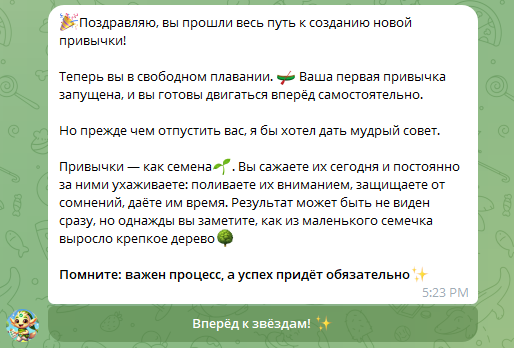
\includegraphics[width=0.6\linewidth]{figures/Bot/bot_onboarding_end.png}
    \caption{Завершающее сообщение онбординга бота «Habiteer»}
    \label{fig:bot_onboarding_end}
\end{figure}

\textit{Отчетность}. На этапе реализации Telegram-бота были добавлены экраны с отчетами, которых не было в бумажном прототипе. Они, в целом, повторяют шаг \ref{th:implement} алгоритма Tiny Habits. Если пользователь не выполнил привычку, он может выбрать одну из трёх причин: «просто забыл», «слишком сложно» или «я больше не хочу эту привычку». При более чем двух пропусках подряд опция «просто забыл» заменяется на «продолжаю забывать» (рис. \ref{fig:report_screens}-а). Если в качестве триггера пользователь выбирал уведомления, то опция «просто забыл» трансформируется в «пропустил уведомление», а «продолжаю забывать» в «продолжаю пропускать уведомления».

\begin{figure}
    \centering
    
\includegraphics[width=0.49\linewidth]{figures/Bot/bot_report.png}
    
\includegraphics[width=0.49\linewidth]{figures/Bot/bot_report_praise.png}
    \caption{(а) — варианты ответа в отчёте при невыполнении привычки; (б) — сообщение с похвалой пользователю}
    \label{fig:report_screens}
\end{figure}

При выборе каждой из опций запускается соответствующая логика:

\begin{itemize}
    \item \textbf{«Просто забыл»} → пользователю предлагается отрепетировать привычку ещё раз.
    \item \textbf{«Продолжаю забывать»} (при более чем двух пропусках подряд) → предлагается изменить поведение-триггер.
    \item \textbf{«Пропустил уведомление»} (доступно, если активированы уведомления) → бот отображает краткое напоминание с призывом не пропускать уведомления в будущем.
    \item \textbf{«Продолжаю пропускать уведомления»} (при активных уведомлениях и более чем двух пропусках подряд) → предлагается изменить тип триггера — привязать привычку к уже существующей рутине.
    \item \textbf{«Слишком сложно»} → предлагается упростить привычку.
    \item \textbf{«Я больше не хочу эту привычку»} → привычка удаляется или откладывается.
\end{itemize}

Если привычка была отмечена как выполненная, бот хвалит пользователя и случайным образом отображает одно из более чем пятидесяти GIF-изображений, связанных с темой празднования и поздравлений (рис. \ref{fig:bot_onboarding_end}-б). Использование переменной награды является важным элементом модели Hook Model, способствующим формированию устойчивой привычки прохождения отчёта \cite{eyal_hooked_2014}.

Помимо ежедневных отчётов, в бота были интегрированы ежемесячные отчёты, направленные на оценку степени автоматичности поведения. Пользователю предлагалось пройти анкету, состоящую из четырёх утверждений, на которые он отвечал по пятибалльной шкале Лайкерта. На основе этих ответов бот рассчитывал показатель SRBAI (Self-Reported Behavioral Automaticity Index), представляющий собой сокращённую версию индекса SRHI (Self-Reported Habit Index)~\cite{gardner_towards_2012}. Для использования в боте автор данной работы самостоятельно адаптировал опросник SRBAI на русский язык.

В зависимости от полученного значения SRBAI выполнялись следующие действия:

\begin{itemize}
    \item \textbf{SRBAI $\geq$ 16} → отслеживание привычки завершалось, и она переносилась в «Зал славы».
    \item \textbf{12 $\leq$ SRBAI $\leq$ 15} → привычка продолжала отслеживаться без изменений.
    \item \textbf{SRBAI $\leq$ 11} → пользователю предлагалось упростить привычку.
\end{itemize}

Также перед прохождением анкеты пользователю предлагалось выбрать срок следующего SRBAI-отчёта: на следующий день или через месяц. Эта функция была добавлена на случай, если пользователь по каким-либо причинам не сможет пройти опрос в текущий день.

\textit{Изменения в разделе «Мои привычки»}. Изменилась логика выбора привычки: в бумажном прототипе пользователь сначала нажимал «изменить привычку», а затем выбирал её номер из списка. В Telegram-боте порядок действий был обратным — сначала необходимо выбрать номер привычки, после чего становятся доступны различные действия с ней. 

\begin{figure}
    \centering
    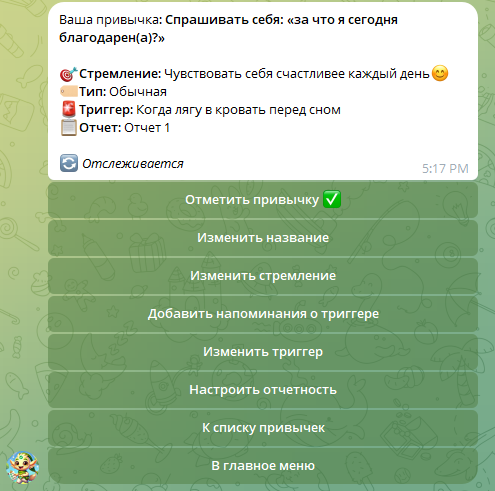
\includegraphics[width=0.6\linewidth]{figures/Bot/bot_habit_info.png}
    \caption{Информация об отслеживаемой привычке}
    \label{fig:bot_habit_info}
\end{figure}

Также был переработан экран информации о привычке: в нём появились дополнительные параметры настройки, касающиеся только выбранной привычки. Пользователь может:
отметить выполнение привычки, изменить тип триггера и сам триггер, добавить или изменить стремление, настроить напоминания о триггере, а также задать параметры отчетности (рис. \ref{fig:bot_habit_info}). Помимо этого, бот отображает основную информацию о привычке: её название, стремление, тип, выбранный триггер, название связанного отчёта, а также текущий статус. Статус может принимать одно из четырёх значений: «не отслеживается», «отслеживается», «отслеживание приостановлено», «ожидает репетиции». Если привычка находится в статусе «отслеживается» и была хотя бы один раз отмечена как выполненная, отображаются также текущая и лучшая серия. При этом пользователь может не только отметить привычку как выполненную, но также приостановить её отслеживание или завершить досрочно — до успешного прохождения SRBAI-отчёта.

\begin{figure}
    \centering
    
\includegraphics[width=0.6\linewidth]{figures/Bot/bot_simplify.png}
    \caption{Уточняющий вопрос бота о выполнимости поведения}
    \label{fig:bot_simplify}
\end{figure}

Кнопка «Улучшить привычку» была переименована в «Начать отслеживать». Изменился и сам процесс начала отслеживания. После выбора типа привычки бот задаёт пользователю уточняющий вопрос: «Сможете ли вы выполнить эту привычку, даже если вы устали или не в настроении?» (рис. \ref{fig:bot_simplify}). Если пользователь отвечает «Нет, выглядит сложно», он переходит на этап упрощения привычки (шаг~\ref{th:simlpify} метода Tiny Habits). Бот предлагает два способа упростить поведение: сделать только первый шаг к желаемому действию или уменьшить объём привычки. 

После ввода упрощённой версии (или если пользователь ответил «Да, смогу»), начинается выбор способа напоминания. На этом этапе формулировка была изменена с термина «триггер» на вопрос: «Как вы будете напоминать себе о привычке?». Такое изменение было сделано по результатам тестирования бумажного прототипа, в ходе которого термин «триггер» вызывал у пользователей затруднения. Дополнительно пользователю объясняется, почему лучше выбрать внешнее поведение в качестве напоминания, а не уведомления: последние могут прийти в неподходящий момент, а телефон — не всегда оказаться под рукой. Сохранение выбора типа триггера важно для универсальности: если пользователь предпочитает старые и проверенные способы, нет причин ограничивать его в этом. 

Далее пользователю предлагается список из десяти случайно выбранных готовых поведений-триггеров. Пользователь может привязать к одному из них свою привычку (шаг~\ref{th:trigger} метода Tiny Habits). Все триггеры распределены по времени суток и контексту: четыре из них относятся к утренним действиям, один — к ситуациям в транспорте, три — к рабочему времени и два — к вечернему периоду. Если ни один из этих триггеров не подходит для пользователя, он может выбрать соответствующую опцию и ввести триггер вручную. Экран репетиции привычки (шаг~\ref{th:repeat} алгоритма) и прикрепления отчёта в целом остался без изменений, за исключением корректировки формулировок.

Также была добавлена возможность создавать вредные и «одноразовые» привычки. Хотя последние по сути представляют собой задачи, а не привычки, формулировка «привычка» была сохранена для поддержания терминологической целостности интерфейса. При работе с вредными привычками пользователю предлагаются три стратегии: удалить или избегать триггер (с помощью действия, устраняющего его, или установки напоминания, помогающего его избежать); и, если первые два варианта недоступны, — усложнить выполнение самой вредной привычки. Для одноразовых действий предусмотрена возможность задать период и время напоминаний.

\textit{Изменения в разделе «подобрать привычку»}. Был обновлён список готовых стремлений: удалены дублирующие по смыслу категории, исключены наименее актуальные, а также добавлены новые, такие как «заботиться о доме» и «помогать людям». Экраны ввода и прояснения стремления, в целом, остались без изменений (шаг \ref{th:aspiration}).

На этапе выбора вариантов поведения (шаг~\ref{th:beh_explore}) пользователь теперь может выбрать опцию «У меня нет идей...». В этом случае ему предлагается список возможных вариантов поведения, сгенерированных с помощью искусственного интеллекта. Пользователь может принять любые из предложенных вариантов или отклонить помощь. Подбор с использованием ИИ осуществляется за кредиты: пользователю ежедневно предоставляется один бесплатный кредит на генерацию.

Сама процедура ввода вариантов поведения также была изменена. Вместо того чтобы вводить их списком, пользователь теперь добавляет варианты по одному. Аналогичные изменения коснулись и этапа оценивания (шаг~\ref{th:beh_eval}): вместо одновременного ввода номеров и оценок пользователь оценивает каждый вариант по отдельности с помощью кнопок от 1 до 10, соответствующих десятибалльной шкале.

После ввода пяти вариантов поведения пользователь может перейти к этапу оценивания или продолжить подбор. В последнем случае у него появляется 10\% вероятность получить дополнительно 3 кредита за расширенный список, превышающий минимально необходимое количество.

\textit{Зал славы.} Раздел «Статистика» был переименован в «Зал славы». Основной причиной переименования стало стремление сохранить простоту реализации: поскольку бот представляет собой MVP, добавление сложной визуальной аналитики и графиков было признано нецелесообразным. Новый формат делает акцент не на количественных показателях, а на достижениях пользователя, что соответствует общей мотивационной направленности интерфейса.

«Зал славы» представляет собой список привычек, которые пользователь успешно завершил. В него входят как полезные привычки, которые удалось внедрить, так и вредные, от которых пользователь отказался. При этом предусмотрена возможность убрать привычку из «Зала славы», чтобы возобновить её отслеживание.

\textit{Изменения в настройках.} Из интерфейса настроек была удалена опция включения и выключения мотивационных сообщений, поскольку такие сообщения не предполагались изначально. Вместо этого на экран настроек была добавлена информация о текущем количестве доступных кредитов. Также появилась возможность изменить часовой пояс. Поскольку Telegram не предоставляет доступ к геолокации пользователя, часовой пояс задавался вручную в начале онбординга. В случае переезда или ошибочного ввода пользователь теперь может самостоятельно скорректировать этот параметр в настройках.

После рассмотрения основных изменений стоит пояснить, почему алгоритм Tiny Habits был реализован в непоследовательной форме: пользователь мог пройти одни шаги, минуя другие, и наоборот. Кроме того, следует отдельно объяснить, почему шаг~\ref{th:beh_crispify} не был включён в реализацию.

«Разрыв» последовательности — то есть ситуация, при которой пользователь проходил шаги 1,2,4 на этапе подбора привычки, а шаги 5–7 уже в разделе «Мои привычки» (при начале отслеживания), — был обусловлен необходимостью соблюсти три ключевых требования, сформулированных в конце первого раздела: простота взаимодействия, гибкость в настройке и минимальное когнитивное и эмоциональное напряжение. Реализация всего алгоритма целиком и сразу могла бы перегрузить пользователя на старте, снизить мотивацию и увеличить вероятность отказа от использования бота.

Что касается шага 3, он не был реализован из-за ограничений интерфейса Telegram-бота: реализовать его простым и удобным способом оказалось невозможно. Этот шаг предполагает пересмотр уже сформулированных вариантов поведения и редактирование тех, что оказались недостаточно конкретными. Для реализации в формате бота потребовалось бы показывать каждый вариант по отдельности и запрашивать у пользователя оценку его чёткости — что сделало бы процесс излишне громоздким и затянутым. Вместо этого акцент на чёткости формулировок был перенесён в текст подсказки, сопровождающей этап брейншторма. В будущем этот шаг будет реализован в мобильном приложении.

\subsubsection{Архитектура}

Telegram-бот разработан на языке Python с использованием Telegram Bot API. Исходный код доступен в репозитории на GitHub: \url{https://github.com/FarmerKarwer/habiteer_bot}. Сам бот доступен по ссылке: \url{https://t.me/habiteer_test_bot}.

Хостинг осуществляется на платформе Yandex Cloud с использованием следующих облачных сервисов:

\begin{itemize}
    \item \textbf{Cloud Functions}, в рамках которых реализованы следующие компоненты:
    \begin{itemize}
        \item \textit{Основная функция}. Обрабатывает входящие запросы от пользователей и реализует большую часть логики бота, за исключением напоминаний и отчётов. Функция выступает в роли event listener'а, получая ввод (сообщения или ответы на кнопки) и формируя ответ. Запросы передаются через API-шлюз.
        \item \textit{Ежедневные отчёты}. Запускается ежеминутно и отвечает за отправку отчётов о привычках. Такой частый интервал позволяет учитывать индивидуальное расписание, заданное пользователями.
        \item \textit{Напоминания о привычках}. Также запускается каждую минуту и проверяет, требуется ли в текущий момент отправить напоминание о выполнении привычки.
        \item \textit{Ежемесячные отчёты}. Отвечает за отправку напоминаний о прохождении SRBAI-отчёта каждые 30 дней.
        \item \textit{Обновление серий привычек}. Запускается ежедневно в полночь по московскому времени и пересчитывает текущие и лучшие серии привычек пользователей.
        \item \textit{Начисление кредитов}. Аналогично предыдущей функции, запускается ежедневно в полночь и добавляет пользователям один кредит на генерацию вариантов поведения с помощью ИИ.
    \end{itemize}
    
    \item \textbf{API-шлюз}. Принимает входящие запросы от Telegram Bot API через вебхук и перенаправляет их в основную облачную функцию.
    
    \item \textbf{Managed Service for YDB}. Бессерверная база данных, используемая для хранения постоянных и временных данных. Структура включает восемь строковых таблиц для долгосрочного хранения и восемь документных таблиц, которые служат кэшем.
    
    \item \textbf{Object Storage}. Предназначен для хранения медиафайлов (изображений и GIF-анимаций), отправляемых пользователям в отчётах.
    
    \item \textbf{Foundation Models}. Генерация вариантов поведения осуществляется с использованием языковой модели Yandex GPT 4 Lite.
    
    \item \textbf{DataLens}. Используется для визуализации и анализа данных, хранящихся в YDB.
\end{itemize}

Для сокращения времени отклика после периодов бездействия была проведена оптимизация холодного старта облачных функций. Во-первых, уменьшено количество внешних зависимостей, а загрузка ресурсоёмких библиотек перенесена на момент их фактического использования (lazy loading). Во-вторых, отключено ограничение пропускной способности YDB, что устранило задержки при резком увеличении нагрузки. Эти меры обеспечили более стабильную и быструю работу системы.

\subsection{Юзабилити-тестирование бота}

Прежде чем приступить к эксперименту, в рамках которого участникам предстояло использовать бота в течение 21 дня, было проведено предварительное юзабилити-тестирование. Его цель заключалась в том, чтобы на раннем этапе выявить технические неполадки и возможные трудности в использовании бота. Это особенно важно, поскольку даже незначительные баги или неудобства интерфейса могут негативно повлиять на пользовательский опыт и привести к досрочному выходу участников из исследования.

В ходе тестирования основное внимание уделялось тому, насколько удобно пользоваться ботом при выполнении ключевых задач. Необходимо было выяснить, какие элементы интерфейса вызывают затруднения, что может быть непонятно без дополнительных пояснений, и какие действия оказываются для пользователей излишне сложными или запутанными.

\subsubsection{Процедура и задачи}

Для оценки удобства и понятности ключевых функций бота были сформулированы исследовательские вопросы. В частности, проверялось:

\begin{itemize}
    \item Корректно ли пользователи вводят названия привычек, и понимают ли они, что речь идёт именно о конкретном повторяющемся поведении?
    \item Насколько ясно сформулированы объяснения в интерфейсе, особенно при запуске отслеживания привычек?
    \item Легко ли пользователям самостоятельно вводить варианты поведения, а затем возвращаться к ним для оценки?
    \item Как именно пользователи проходят онбординг и с чего начинают работу с ботом после первого запуска?
    \item Какое представление о боте у них формируется и как они его воспринимают?
\end{itemize}

Сбор данных осуществлялся в качественном формате. Качественная часть анализа включала комментарии пользователей, зафиксированные в процессе тестирования, а также данные из последующих follow-up интервью.

Сначала каждому участнику случайным образом назначались четыре задания (за исключением онбординга, который проходили все участники). Затем, по мере проведения исследования, оставшиеся сценарии были равномерно распределены между участниками, чтобы обеспечить полное покрытие всех вариантов.

Ниже приведён список всех сценариев:

\begin{enumerate}
    \item \textit{Онбординг и первое взаимодействие.} Участник переходил по ссылке на бота и впервые запускал его. Задача — пройти вводный этап и прокомментировать, насколько понятны инструкции и структура интерфейса.
    \item \textit{Добавление новой привычки.} Участнику предлагалось представить, что он решил начать регулярно бегать, используя чат-бот. Необходимо было добавить соответствующую привычку и описать, какие действия для этого предпринимаются.
    \item \textit{Формулировка и отслеживание привычки.} Участнику предлагалось ввести новую привычку (например, изучение английского языка), запустить её отслеживание и описать свои действия.
    \item \textit{Подбор привычки с нуля.} Участнику предлагалось представить, что он хочет начать работать над какой-то полезной привычкой, но пока не знает точно, какой именно.
    \item \textit{Добавление нежелательной привычки.} Участник должен был внести привычку, от которой хочет избавиться (например, «отвлекаться на соцсети»), и начать её отслеживание.
    \item \textit{Раннее выполнение привычки.} Допускалась ситуация, в которой привычка (например, прогулка) была выполнена до прихода напоминания. Участнику нужно было найти способ отметить её как выполненную.
    \item \textit{Изменение времени уведомлений.} Участнику предлагалось представить, что напоминания приходят в неудобное время. Он должен был изменить настройки времени уведомлений.
    \item \textit{Реакция на устоявшуюся привычку.} Участнику предлагалось смоделировать ситуацию, когда привычка уже укоренилась и выполняется автоматически. Требовалось решить, как поступить с продолжающимися напоминаниями.
\end{enumerate}

\subsubsection{Участники}

Так как тестирование носило предварительный характер, было решено обойтись небольшим числом участников без деления на сегменты. Оптимальным решением стал метод удобной выборки (convenience sampling).

Набор участников происходил через общий чат одногруппников, куда была размещена ссылка на запись через Calendly для онлайн-встреч в Google Meet. Также к участию были приглашены друзья и знакомые автора. Такой подход позволил быстро собрать начальную группу из четырех человек для проведения тестирования в сжатые сроки.

\subsubsection{Результаты}

\paragraph{Корректно ли пользователи вводят названия привычек, и понимают ли они, что речь идёт именно о конкретном повторяющемся поведении?}

В целом пользователи корректно вводили названия привычек. Многие обращали внимание на подсказку, где подчёркивалось, что вводимое действие должно быть конкретным и повторяющимся. 

\paragraph{Насколько ясно сформулированы объяснения в интерфейсе, особенно при запуске отслеживания привычек?}

Участники отмечали, что инструкции в интерфейсе не всегда были однозначными. Некоторые участники испытывали затруднения при ручном вводе привычек: не всегда было понятно, что именно требуется — поведение, стремление или привычка. Термины вроде \textit{стремление}, \textit{поведение}, \textit{привычка} и \textit{отчёты} вызывали путаницу и снижали точность ввода. Кроме того, был выявлен баг, позволявший отметить привычку как выполненную, даже если она выполнялась не в тот день. Например, на экране репетиции привычки некоторые пользователи полагали, что привычку следует выполнять 5–7 дней, а не 5–7 раз подряд. 

\paragraph{Легко ли пользователям самостоятельно вводить варианты поведения, а затем возвращаться к ним для оценки?}

Был обнаружен баг: если пользователь вводил пять вариантов поведения, бот переставал работать. Кроме того, возврат к экрану с готовыми привычками вызывал сбой.

\paragraph{Как именно пользователи проходят онбординг и с чего начинают работу с ботом после первого запуска?}

Онбординг в целом проходил успешно, однако предложенная по умолчанию привычка благодарности не всегда соответствовала целям пользователей. Также было отмечено, что при пропуске информации не всегда можно было вернуться к предыдущим шагам.

\paragraph{Какое представление о боте сформировалось у участников и как они его воспринимают?}

В целом участники воспринимали бота умеренно положительно: он вызывал доверие и воспринимался как полезный инструмент. Отдельные пользователи отмечали, что бот создаёт ощущение поддержки, особенно на начальных этапах взаимодействия. В то же время были зафиксированы трудности, связанные с терминологией и логикой интерфейса, а также выявлены три бага. Один из них оказался критическим: из-за него облачная функция прекращала выполнение. Несмотря на указанные проблемы, общее впечатление от использования бота оставалось скорее благожелательным.

\subsubsection{Выводы}

По результатам юзабилити-тестирования в интерфейс и функциональность Телеграм-бота были внесены следующие изменения:

\begin{itemize}
\item Исправлены выявленные баги и ошибки интерфейса, препятствовавшие стабильной работе. В частности, реализован универсальный хандлер ошибок, обеспечивающий продолжение выполнения облачной функции даже при возникновении нестандартных ситуаций.
\item Уточнены формулировки в пользовательских инструкциях для снижения неоднозначности терминов.
\item На всех этапах онбординга добавлены кнопки «Назад» для обеспечения гибкости навигации.
\item Добавлена кнопка «Мне нужно что-то другое» в случае, если предложенная по умолчанию привычка благодарности не подходит пользователю.
\item Сокращён текст на ряде экранов: например, пояснение по репетиции привычки теперь скрыто за отдельной кнопкой, позволяющей просмотреть дополнительную информацию при необходимости.
\end{itemize}

Как и в случае с тестированием бумажного прототипа, данное исследование характеризуется рядом существенных ограничений. Выборка участников была небольшой и формировалась из круга друзей и знакомых автора, что не позволяет считать её репрезентативной для широкой популяции. Все участники были предварительно знакомы с методом Tiny Habits, однако никто из них не применяет его на практике. Влияние данных ограничений необходимо учитывать при анализе и интерпретации результатов.

\subsection{Рандомизированный эксперимент}

Первым вопросом данного раздела был: какая должна быть логика у приложения? В предыдущем подразделе мы, в целом, ответили на этот вопрос. В этом же подразделе мы попробуем ответить на следующий вопрос: насколько предложенная логика может обеспечить более эффективное формирование привычек, а также насколько она удобна в использовании по сравнению с лучшими существующими аналогами?

Для получения исчерпывающего ответа на этот вопрос может подойти рандомизированное контролируемое испытание (РКИ), поскольку этот метод позволяет устанавливать причинно-следственные связи. Результаты РКИ также могут быть использованы для постановки бенчмарков удобства использования будущего приложения.

Исследовательские вопросы:

\begin{itemize}
    \item Насколько бот лучше или хуже помогает формировать привычки по сравнению с другими популярными приложениями?
    \item Есть ли заметные различия в удовлетворённости между пользователями бота и других приложений?
    \item Насколько удобно пользоваться ботом по сравнению с аналогами?
    \item С какими трудностями могут столкнуться пользователи бота?
\end{itemize}

Поскольку рекрутинг участников и их вознаграждение сопряжены с существенными затратами, автор данной работы решил начать с проведения пилотного рандомизированного контролируемого эксперимента. Задачами пилота являются оценка осуществимости рекрутинга, уровня вовлечённости участников, адекватности применяемой методики, а также сбор данных для уточнения необходимого объёма выборки и параметров дизайна основного исследования.

\subsubsection{Участники}

Рекрутинг участников был проведён из двух источников: 1) контактов, которые оставляли участники, изъявившие желание участвовать в дальнейших исследованиях после прохождения опроса (см. подраздел \ref{Survey}); 2) e-mail рассылки студентам НИУ ВШЭ. Участникам предлагалось пройти опрос, в ходе которого были собраны baseline-характеристики и определено их право на участие. Для определения канала привлечения каждого участника были созданы два идентичных опроса в системе JotForm — по одному для каждого источника.

Критерии включения участников были следующими: 1) возраст 16 лет и старше; 2) наличие смартфона с доступом в интернет; 3) желание внедрить хотя бы одну полезную привычку, связанную с уменьшением стресса; 4) наличие аккаунта в Телеграм. Критерии исключения: 1) знакомство с Tiny Habits или опыт применения этого метода; 2) желание исключительно избавиться от вредных привычек; 3) использование приложений для формирования привычек; 4) уже внедрённая привычка благодарности.

Поскольку исследование носит пилотный характер, его основной целью была не статистическая значимость результатов, а оценка осуществимости проведения эксперимента. В связи с этим точный расчёт размера выборки на основе мощности критерия (power analysis) не проводился. Вместо этого ориентиром послужило приблизительное количество участников, которых реально привлечь. Согласно предварительному опросу, 30 человек выразили интерес к участию, и при оптимистичном сценарии ожидалось, что около 20 из них действительно согласятся участвовать. В случае меньшего отклика планировалось дополнительно привлечь участников с помощью e-mail рассылки. Таким образом, ожидаемый общий размер выборки составлял 20 человек.

\subsubsection{Дизайн эксперимента}

Было проведено рандомизированное параллельное контролируемое испытание. Участники были случайным образом распределены на тестовую и контрольную группы. Рандомизация происходила следующим образом: в конце анкеты скрытно генерировалось случайное число от 0 до 100 с непрерывным равномерным распределением. Если число было меньше 50 — участник попадал в контрольную группу, если больше — в тестовую. По завершении baseline-опроса участники перенаправлялись по ссылке на один из двух опросов в зависимости от группы.

\subsubsection{Вмешательство}

Участники экспериментальной группы указывали свой username в Telegram (если он отсутствовал, его необходимо было создать), что позволяло отличить их от посторонних пользователей и обеспечить корректную персонализацию взаимодействия. Далее участники получали вводную инструкцию через Telegram, в которой сообщалось, что в течение 21 дня им предстоит формировать привычку благодарности с помощью Telegram-бота «Habiteer».

Инструкция содержала приветствие, краткое описание целей исследования и важности привычки благодарности, а также пошаговое объяснение участия. Участникам предлагалось ежедневно отмечать выполнение привычки, используя интерфейс бота. Если выполнение не удалось, они могли оставить поле пустым либо — при наличии включённой функции — указать причину в формате отчёта.

В течение всего 21-дневного периода исследовательская группа не вмешивалась в процесс, однако участникам предоставлялась возможность связаться с организаторами в случае вопросов или затруднений.

По окончании 21-дневного периода бот автоматически отправлял пользователю сообщение со ссылкой на финальную анкету. В анкете оценивались уровень автоматичности целевой привычки, удобство взаимодействия с ботом и общий уровень удовлетворённости. Также участники могли по желанию оставить отзыв о работе бота. В качестве награды за заполнение анкеты предоставлялась ссылка на подборку из 40 электронных и 18 аудиокниг по саморазвитию — та же, что использовалась и для интервью (см. подраздел \ref{Interview}).

\subsubsection{Компаратор}

Участникам контрольной группы предлагалось выбрать одно из трёх популярных мобильных приложений для формирования привычек: Habitica (доступно в Google Play и App Store), Habit Tracker – Habit Diary (Google Play), или Hizo (Google Play и App Store). Эти приложения были выбраны на основании их популярности, высокого пользовательского рейтинга (выше 4.5) и поддержки русского языка. Несмотря на различия в функциональности, это не рассматривалось как ограничение: целью было сравнение эффективности предлагаемого Telegram-бота с существующими решениями вне зависимости от их особенностей.

После выбора приложения участникам предоставлялась инструкция, поясняющая, как использовать его для внедрения привычки благодарности. В инструкции предлагалось выбрать формулировку привычки (например, «За что я сегодня благодарен(а)?») и ежедневно отмечать её выполнение в течение 21 дня. Участники могли использовать любое удобное представление прогресса, встроенное в выбранное приложение.

Также участники получали ссылку на отдельного Telegram-бота (не связанного с Habiteer), который по завершении 21-дневного периода автоматически направлял им финальную анкету. В ней оценивались уровень автоматичности целевой привычки, удобство взаимодействия с приложением и общий уровень удовлетворённости. Участники могли по желанию оставить отзыв о работе приложения. Заполнение анкеты поощрялось — в качестве награды предоставлялась ссылка на 40 электронных и 18 аудиокниг по теме саморазвития (см. подраздел \ref{Interview}).

На протяжении всего периода исследования вмешательство со стороны исследовательской группы не осуществлялось, однако участники могли при необходимости обращаться за поддержкой.

\subsubsection{Исходы}

Основными исходами в проведённом исследовании являлись изменения в шкале автоматичности привычек (Self-Report Behavioral Automaticity Index, SRBAI) и количество выполнений целевой привычки в течение 21-дневного периода. Изменения в SRBAI позволили оценить степень автоматизации поведения, тогда как частота выполнения привычки отражала фактическую поведенческую активность участников.

Вторичными исходами выступали субъективная оценка удобства использования приложения на основе шкалы System Usability Scale (SUS), уровень удовлетворённости, измеренный с помощью Customer Satisfaction Index (CSI), а также индекс лояльности (Net Promoter Score, NPS), отражающий готовность участников рекомендовать использованный инструмент.

Дополнительно были собраны демографические и контекстуальные характеристики, потенциально влияющие на исходы, включая пол, возраст, а также предварительный опыт использования мобильных приложений и платформы Telegram. Эти данные фиксировались на начальном этапе исследования и впоследствии использовались в анализе.

\subsubsection{Анализ данных}

Для анализа данных была собрана дескриптивная статистика, описывающая характеристики участников исследования, включая демографические параметры и поведенческие показатели. Обработка данных и расчёты осуществлялись с использованием библиотек Python, в частности, SciPy и statsmodels.

Анализ проводился по принципу intention-to-treat, что предполагает включение в итоговый анализ всех рандомизированных участников, независимо от степени их участия в интервенции — включая тех, кто не воспользовался ботом, преждевременно завершил участие или не заполнил итоговую анкету.

Ввиду ограниченного объёма выборки, проведение продвинутого (инферентного) статистического анализа не предусматривалось; основной акцент был сделан на описательных результатах и выявлении общих тенденций.

Информация о ключевых метриках и соответствующих методах анализа представлена в таблице \ref{tab:rct_outcomes}:

\begin{table}[h!]
\normalsize
\centering
\caption{Методы анализа данных по каждому из исходов}
\label{tab:rct_outcomes}
\begin{tabular}{|p{5cm}|p{8cm}|}
\hline
\textbf{Исход} & \textbf{Метод анализа} \\
\hline
Изменения в SRBAI & Разница в средних/медианах, размах \\
\hline
Частота выполнения привычки & Медиана, межквартильный размах (IQR) \\
\hline 
SUS & Медиана, межквартильный размах (IQR) \\
\hline 
NPS & Среднее \\
\hline  
CSI & Доля поставивших 4/5 и 5/5 \\
\hline
\end{tabular}
\end{table}

\subsubsection{Результаты}

\textit{Характеристики и отток участников}. Первоначально приглашения к участию в исследовании были отправлены 30 участникам, ранее выразившим заинтересованность в участии в научных опросах. Из них согласие дало 16 человек. Для увеличения выборки была организована e-mail-рассылка среди студентов НИУ ВШЭ. Рассылка проводилась итеративно, с учётом текущего количества респондентов, прошедших опрос по ссылке. В результате были приглашены 239 студентов, однако лишь 7 из них согласились поучаствовать. 

Всего 23 участника прошли baseline-опрос и были оценены на соответствие критериям включения. Из них 8 человек были исключены в связи с несоответствием критериям: четверо уже использовали приложения для формирования привычек, двое практиковали благодарность до начала исследования, один не имел аккаунта в Telegram, а ещё один отказался внедрять новую привычку, направленную на снижение стресса.

Из оставшихся 15 участников 8 были рандомизированы в тестовую группу. Один из них прекратил участие и не предоставил финальных данных; контакт с ним установить не удалось. Тем не менее, его базовые данные были включены в итоговый анализ. Семь участников были распределены в контрольную группу; все они завершили участие в исследовании и предоставили полный набор данных.

В итоговую выборку вошли 15 участников, среди которых преобладали женщины — 12 человек (80 \%), в то время как мужчин было 3 (20 \%). Средний возраст участников составил 26,8 лет (26,5 года в тестовой группе и 27,1 года в контрольной) — самому младшему участнику было 19 лет, а самому старшему — 35.

Большинство участников активно использовали мобильные приложения: 10 человек (67 \%) сообщили, что делают это постоянно, 4 (27 \%) — часто, и лишь 1 участник (6 \%) — редко.

Telegram также был широко распространён среди участников. В отношении длительности использования мессенджера: 13 человек (87 \%) использовали его более одного года, и 2 (13 \%) — от 6 до 12 месяцев. По частоте использования Telegram 11 участников (73 \%) указали, что пользуются им постоянно, 3 (20 \%) — часто, и 1 (7 \%) — почти никогда.

Распределение по основным характеристикам между тестовой (N = 8) и контрольной (N = 7) группами было сопоставимым, что свидетельствует о хорошем балансе после рандомизации (см. таблицу \ref{tab:rct_groups}).

\begin{table}[ht]
  \centering
  \caption{Баланс характеристик после распределения}
  \label{tab:rct_groups}
  \begin{tabular}{@{} l c c @{}}
    \toprule
    Параметр 
      & \parbox[c]{4cm}{\centering Тестовая\\группа (N = 8)} 
      & \parbox[c]{4cm}{\centering Контрольная\\группа (N = 7)} \\
    \midrule
    Пол 
      & Жен: 6 (75\%) / Муж: 2 (25\%) 
      & Жен: 6 (86\%) / Муж: 1 (14\%) \\

    Частота Telegram 
      & \parbox[t]{4cm}{Постоянно: 6\\ Часто: 1\\ Почти никогда: 1} 
      & \parbox[t]{4cm}{Постоянно: 5\\ Часто: 2\\ Редко: 0} \\

    Давность Telegram 
      & \parbox[t]{4cm}{Более 1 года: 6\\ 6--12 мес.: 2} 
      & \parbox[t]{4cm}{Более 1 года: 7\\ 6--12 мес.: 0} \\

    Возраст (средний) 
      & 26,5 года 
      & 27,1 года \\

      Канал 
      & \parbox[t]{4cm}{Контакты из опроса: 4\\ E-mail рассылка студентам ВШЭ: 4} 
      & \parbox[t]{4cm}{Контакты из опроса: 5\\ E-mail рассылка студентам ВШЭ: 2}  \\
    Выбывание 
      & 1 
      & 0 \\
    \bottomrule
  \end{tabular}
\end{table}

\textit{Автоматичность привычек}. Участники тестовой группы продемонстрировали немного более высокий уровень автоматизации привычки по шкале SRBAI по сравнению с контрольной группой (в среднем 3.3 против 3.0), что соответствует предполагаемому направлению эффекта. Однако размер выборки крайне мал, и эта разница не позволяет делать статистически обоснованные выводы. Полученные данные можно рассматривать лишь как предварительное наблюдение, требующее подтверждения в последующих исследованиях с более крупной выборкой.

\textit{Удобство использования}. В контрольной группе 2 человека выбрали Habitica, 2 — Hizo, и 3 участника — Habit Tracker – Habit Diary. По шкале SUS контрольные приложения (в среднем) получили более высокую оценку (в среднем 75 балла против 68 в тестовой группе). Аналогично, показатель лояльности пользователей (NPS) оказался выше в контрольной группе (8 против 7,1). 

Дополнительно стоит отметить, что один из участников оставил отзыв в финальной форме, в котором указал на ограничение функциональности бота: в нём отсутствовала возможность пропустить выполнение привычки на день, если не было физической возможности её выполнить. 

Индекс потребительской удовлетворённости (Customer Satisfaction Index, CSI), отражающий долю участников, поставивших высокую оценку (4 или 5 баллов из 5), составил 86\% в тестовой группе (6 из 7 участников) и 75\% в контрольной (5 из 7). Эти показатели свидетельствуют о положительном восприятии бота и приложений участниками. Однако, учитывая крайне малый объём выборки, любые количественные сравнения между группами следует рассматривать как предварительные и интерпретировать с осторожностью. Полученные результаты могут служить ориентиром для дальнейшего тестирования, но не являются достаточной основой для окончательных выводов.

\begin{table}[h!]
\centering
\normalsize
\caption{Сравнение параметров между тестовой и контрольной группами}
\begin{tabular}{|l|c|c|}
\hline
\textbf{Параметр} & \textbf{Тестовая (N=8)} & \textbf{Контрольная (N=7)} \\
\hline
SRBAI (среднее, max=5) & \textbf{3.3 ± 0.5} & 3.0 ± 0.4 \\
\hline
SUS (max=100) & 68 (медиана: 65, IQR: 60–75) & \textbf{75} (медиана: 76, IQR: 70–80) \\
\hline
NPS (max=10) & 7.1 ± 1.2 & \textbf{8.0 ± 0.8} \\
\hline
CSI (доля 4/5 и 5/5) & \textbf{86\% (6/7)} & 75\% (5/7) \\
\hline
Выбывание & 1 участник & 0 \\
\hline
\end{tabular}
\end{table}

\subsubsection{Выводы}

Пилотное исследование подтвердило осуществимость предложенной методологии и выявило ряд важных организационных и содержательных аспектов, которые необходимо учесть при планировании масштабного РКИ. Один из ключевых уроков касается стратегии рекрутинга: персонализированные подходы, основанные на предварительном взаимодействии (например, через опросы), оказались значительно эффективнее массовых коммуникаций. Это указывает на важность налаженного контакта с аудиторией ещё до начала вмешательства.

Высокий уровень завершённости среди участников (93\%) подтверждает, что 21-дневный формат вмешательства является для них реалистичным и приемлемым.

Предварительные данные об эффективности вмешательства демонстрируют некоторую положительную динамику: в тестовой группе зафиксировано незначительное увеличение уровня автоматичности поведения по шкале SRBAI. При этом масштабы изменений не позволяют делать выводы об эффективности бота в формировании привычек. В то же время контрольные приложения получили более высокие оценки по показателям удобства использования и пользовательской лояльности. Это, вероятно, связано не только с их функциональной насыщенностью и большей привычностью интерфейсов, но и с более проработанным визуальным и интерактивным дизайном по сравнению с Telegram-ботом, который обладает ограниченными возможностями кастомизации и навигации.

В целом, полученные данные указывают на потенциальную перспективность использования Telegram-бота, основанного на Tiny Habits, как инструмента поддержки формирования привычек. Высокий уровень удовлетворённости участников (CSI = 86\%) и умеренная положительная динамика по показателю автоматичности поведения позволяют рассматривать данный подход как обоснованный для дальнейшего изучения. Вместе с тем, ограниченность выборки, предварительный характер результатов и отсутствие объективных метрик не позволяют делать окончательные выводы об эффективности вмешательства. Для верификации наблюдаемых эффектов и оценки устойчивости изменений требуется проведение более масштабного исследования с улучшенным дизайном и контролем ключевых переменных.

\subsubsection{Ограничения}

Проведённое пилотное исследование сопровождается рядом существенных ограничений, которые необходимо учитывать при интерпретации полученных результатов. В первую очередь, ограниченный объём выборки и выраженный гендерный дисбаланс (80\% женщин) снижают возможность обобщения данных на более широкую популяцию. Вместе с тем, такой дисбаланс может частично отражать особенности самой целевой аудитории, в которой действительно может преобладать женская доля. Кроме того, рекрутинг участников осуществлялся через ограниченные каналы — преимущественно среди респондентов предыдущего опроса и студентов НИУ ВШЭ, — что повышает риск выборочного смещения и ограничивает внешнюю валидность исследования.

Отсутствие статистической значимости наблюдаемых различий объясняется недостаточной мощностью исследования: по результатам постфактум-расчёта, минимально необходимый размер выборки составляет не менее 60 участников на каждую группу при стандартных параметрах ($\alpha = 0{,}05$, $\beta = 0{,}2$). Это подчёркивает необходимость расширения выборки и более строгого дизайна в будущих этапах.

Дополнительные сложности связаны с потенциальным влиянием неучтённых факторов — например, вариативностью уровня вовлечённости участников при использовании разных типов интерфейсов (приложения и Telegram-бот), что могло повлиять как на восприятие вмешательства, так и на выраженность поведенческих изменений. 

Также, отметим, что несмотря на соответствие продолжительности вмешательства (21 день) минимально рекомендованному периоду формирования привычек \cite{lally_how_2010}, столь короткий горизонт наблюдения не позволяет оценить устойчивость достигнутых изменений и долговременность эффектов.

Кроме того, ключевые показатели — автоматичность поведения (SRBAI) и удобство использования интерфейса (SUS) — оценивались исключительно на основе самоотчётов, что увеличивает вероятность искажений (например, связанных с субъективной интерпретацией вопросов). Отдельно следует отметить, что перевод опросника SRBAI на русский язык выполнялся автором исследования, не являющимся специалистом в области психометрии или психологии поведения, что может повлиять на точность интерпретации результатов. Отсутствие объективных поведенческих метрик, таких как данные о взаимодействии с интерфейсом, ограничивает надёжность и валидность выводов.

На основе вышеуказанных ограничений можно выделить следующие направления оптимизации методологии будущих исследований:

\begin{itemize}
    \item применение стратифицированной рандомизации для балансировки ключевых демографических характеристик между группами;
    \item внедрение объективных метрик (например, лог-файлов активности) для дополнения самоотчётных данных;
    \item проведение качественного анализа отзывов участников с целью выявления скрытых барьеров и факторов, влияющих на вовлечённость.
    \item расширение временного горизонта исследования для оценки устойчивости сформированных изменений;
    \item использование официально адаптированных и валидированных русскоязычных версий психометрических шкал, либо проведение процедуры перекрёстной валидации перевода;
\end{itemize}

\subsection{Итоги раздела}

В данном разделе была разработана логика Telegram-бота на основе метода Tiny Habits, проведено тестирование прототипов и экспериментальная оценка его эффективности. Также в разделе рассматривались два ключевых вопроса:

\begin{enumerate}
    \item Какая должна быть логика у приложения?
    \item Насколько предложенная логика может обеспечить более эффективное формирование привычек и быть удобной в использовании по сравнению с существующими аналогами?
\end{enumerate}

На первый вопрос был получен следующий ответ: логика приложения должна строиться на пошаговом алгоритме метода Tiny Habits, но реализовываться не в строго линейной форме, а адаптивно — с учётом ограничений интерфейса, принципов минимизации когнитивной нагрузки и предпочтений пользователей. Для этого целесообразно структурировать алгоритм Tiny Habits на следующие логические блоки:

\begin{itemize}
    \item \textbf{Онбординг}: вводный этап, который не только знакомит пользователя с принципами метода, но и выполняет мотивационную функцию. Он помогает снизить когнитивный барьер на старте взаимодействия, плавно вовлекая пользователя в структуру приложения и подготавливая его к формированию привычек.
    \item \textbf{Подбор привычки}, где реализуются шаги 1–4: прояснение стремления, генерация и уточнение вариантов поведения, а также их оценка.
    \item \textbf{Добавление привычки и её настройка}, где реализуются шаги 5–7: упрощение поведения, подбор триггера и репетиция. При этом важно предусмотреть возможность добавления привычки отдельно, с последующей поэтапной настройкой по желанию.
    \item \textbf{Отчёты}, соответствующие шагу 8, — они позволяют отслеживать выполнение привычки и вносить корректировки, если выполнение нарушается.
\end{itemize}

Такое разбиение позволяет сохранить ключевые принципы метода, обеспечивая пользователю более гибкий и естественный путь прохождения через этапы формирования привычки.

Что касается второго вопроса, то однозначных выводов сделать пока нельзя, так как проведённое исследование носит пилотный характер и имеет ряд методологических ограничений. Тем не менее, предварительные данные позволяют предполагать, что предложенная логика может быть сопоставима по эффективности с подходами, реализованными в популярных приложениях. Пользователи Telegram-бота продемонстрировали умеренно высокие показатели автоматизации поведения и удовлетворённости. В то же время, оценки удобства и пользовательской лояльности оказались несколько ниже, чем у мобильных аналогов — вероятно, из-за ограниченного визуального и интерактивного потенциала Telegram-платформы.

Таким образом, логика приложения показала свою реалистичность и потенциальную применимость, но требует дальнейшего тестирования и доработки. Предварительные результаты выглядят обнадеживающе, однако для обоснованных выводов о сравнительной эффективности необходимо проведение масштабного рандомизированного эксперимента с участием более широкой и разнообразной аудитории.

\newpage

\section{Разработка интерфейса и итоговое тестирование}

\subsection{Обзор раздела}

В первом разделе были сформулированы основные требования к разработке приложения. Во втором — на основе этих требований и метода Tiny Habits — была создана логика работы, реализованная в виде Telegram-бота. Этот раздел завершает работу: в нём представлен прототип пользовательского интерфейса приложения \textit{Habiteer}, а также проведена его оценка с точки зрения восприятия целевой аудиторией и удобства использования.

Раздел включает:
\begin{itemize}
    \item разработку прототипа на основе ранее описанной логики;
    \item описание функционала и основных пользовательских сценариев;
    \item тестирование интерфейса с участием представителей целевой аудитории;
    \item анализ результатов и выводы о качестве взаимодействия с приложением.
\end{itemize}

Цель этого этапа — проверить, насколько интерфейс приложения соответствует потребностям пользователей, обеспечивает понятную навигацию и поддерживает процесс формирования привычек. Кроме того, на основе полученной обратной связи определяются возможные направления для его улучшения.

\subsection{Дизайн прототипа приложения}

Разработка прототипа интерфейса началась с выбора инструмента. Для проектирования использовалась платформа Figma, которая позволила быстро создать интерактивный прототип, отражающий ключевые сценарии взаимодействия. Выбор пал на Figma благодаря её гибкости, поддержке совместной работы и возможности создания кликабельных прототипов, что особенно важно для предварительного тестирования.

В процессе проектирования особое внимание уделялось простоте и удобству использования. Интерфейс строился на принципах визуальной ясности и минимализма: все элементы — от структуры экранов до формулировок — были направлены на то, чтобы пользователь легко ориентировался в приложении без перегрузки вниманием.

Визуальный стиль подчёркивает эти принципы. Он выдержан в спокойной, лаконичной манере, способствующей комфортному восприятию. Основной акцент сделан на зелёный цвет как символ роста и движения вперёд. Он используется в ключевых элементах — кнопках, индикаторах и визуальных акцентах — формируя целостный и узнаваемый образ.

При создании логотипа учитывались замечания, полученные в ходе пользовательского интервью. Один из участников отметил, что иконка приложения должна быть хорошо различимой среди других — особенно на загруженном экране смартфона. Это наблюдение было учтено при разработке визуального образа: логотип представляет собой простой, легко узнаваемый силуэт ростка — символ формирования привычек. Ярко-зелёный фон помогает ему выделяться на экране и оставаться читаемым даже в уменьшенном формате.

Иллюстрации, типографика и визуальная иерархия подобраны таким образом, чтобы поддерживать лёгкую и доброжелательную атмосферу, не отвлекая от основного действия. Такой подход делает взаимодействие с интерфейсом естественным и поддерживающим — что особенно важно в контексте формирования привычек.

Рассмотрим функционал приложения и основные пользовательские сценарии более подробно.

\textit{Онбординг}.

\textit{Подбор привычки}.

\textit{Раздел: «привычки»}.

\textit{Раздел: «путь»}.

\textit{Раздел: «статистика»}.

\textit{Раздел: «настройки»}.

\textit{Отчетность}.

\subsection{Юзабилити-тестирование прототипа}
[Цель и исследовательские вопросы]

Для выявления проблем в понимании и использовании интерфейса, а также оценки общего пользовательского восприятия, были сформулированы следующие исследовательские вопросы:

\begin{enumerate}
  \item Насколько понятно пользователю объяснение интерфейса в целом?
  \item Понимает ли пользователь, что означает термин «отрепетировать привычку»?
  \item Насколько понятно объяснение при выборе триггера?
  \item Ясна ли пользователю формулировка «как сделать поведение чётким»?
  \item Насколько легко пользователю добавить новую привычку?
  \item Понимает ли пользователь, что обозначают стадии формирования привычки?
  \item Ясен ли смысл раздела «Зал славы»?
  \item Понимает ли пользователь, что означает «возвращение привычек» в зале славы?
  \item Понимает ли пользователь, как расставлять варианты поведения по порядку?
  \item Какое общее впечатление у пользователя от раздела «Статистика»?
  \item Ясен ли смысл раздела «Архив брейнштормов»?
  \item В каких местах интерфейса пользователи не понимают, что от них требуется?
  \item Какую траекторию проходят пользователи во время онбординга?
  \item Какое впечатление производит онбординг?
  \item Как воспринимается пользователями раздел «Путь»?
  \item Какое впечатление производит процесс подбора привычки?
  \item По какой траектории пользователи начинают отслеживать привычку?
  \item Понимает ли пользователь, что такое «режим гика» и зачем он нужен?
  \item Понимает ли пользователь, как отметить привычку задним числом?
  \item Насколько легко пользователю найти следующие функции:
    \begin{itemize}
      \item режим отпуска;
      \item пропуск привычки;
      \item настройка или отключение времени отчёта;
      \item завершение отслеживания привычки.
    \end{itemize}
  \item Какое впечатление производит процесс прохождения отчёта?
  \item Какое общее представление о приложении складывается у пользователя на основе прототипа? Что он думает о нём?
\end{enumerate}

\subsubsection{Процедура и задачи}

Для оценки удобства использования интерфейса было проведено качественное модерируемое юзабилити-тестирование summative-типа с использованием протокола think-aloud. Каждая сессия длилась от 45 до 60 минут.

В исследовании использовался within-subjects design, при котором все участники выполняли один и тот же набор задач. Чтобы избежать эффекта обучения и повысить надёжность результатов, порядок некоторых заданий был рандомизирован.

Все участники начинали тестирование с процедуры онбординга, что позволило стандартизировать начальную точку взаимодействия. Сессии проводились удалённо с использованием видеосвязи через платформу «Яндекс.Телемост».

\subsubsection{Участники}

\subsubsection{Результаты}

\subsubsection{Выводы}

\subsubsection{Ограничения}

\subsection{Итоги раздела}

\section{Заключение}\label{sec6}

\backmatter

\bmhead{Acknowledgements}

Acknowledgements are not compulsory. Where included they should be brief. Grant or contribution numbers may be acknowledged.

Please refer to Journal-level guidance for any specific requirements.

\begin{appendices}

\section{Анкета опроса}\label{secA1}


%%=============================================%%
%% For submissions to Nature Portfolio Journals %%
%% please use the heading ``Extended Data''.   %%
%%=============================================%%

%%=============================================================%%
%% Sample for another appendix section			       %%
%%=============================================================%%

%% \section{Example of another appendix section}\label{secA2}%
%% Appendices may be used for helpful, supporting or essential material that would otherwise 
%% clutter, break up or be distracting to the text. Appendices can consist of sections, figures, 
%% tables and equations etc.

\end{appendices}

%%===========================================================================================%%
%% If you are submitting to one of the Nature Portfolio journals, using the eJP submission   %%
%% system, please include the references within the manuscript file itself. You may do this  %%
%% by copying the reference list from your .bbl file, paste it into the main manuscript .tex %%
%% file, and delete the associated \verb+\bibliography+ commands.                            %%
%%===========================================================================================%%

\bibliography{sn-bibliography}% common bib file
%% if required, the content of .bbl file can be included here once bbl is generated
%%\input sn-article.bbl

\end{document}
